%%%%%%%%%%%%%%%%%%%%%%%%%%%%%%%%%%%%%%%%%%%%%%%%%%%%%%%%%%%%%%%%%%%%%%%%%%%%%%%%%%%%%%%%%%%%%%%%%%%%%%%%%%%%%%%%%%%%%%%%%%%%%%%%%%%%%%%%%%%%%%%%%%%%%%%%%%%
% This is just an example/guide for you to refer to when submitting manuscripts to Frontiers, it is not mandatory to use Frontiers .cls files nor frontiers.tex  %
% This will only generate the Manuscript, the final article will be typeset by Frontiers after acceptance.   
%                                              %
%                                                                                                                                                         %
% When submitting your files, remember to upload this *tex file, the pdf generated with it, the *bib file (if bibliography is not within the *tex) and all the figures.
%%%%%%%%%%%%%%%%%%%%%%%%%%%%%%%%%%%%%%%%%%%%%%%%%%%%%%%%%%%%%%%%%%%%%%%%%%%%%%%%%%%%%%%%%%%%%%%%%%%%%%%%%%%%%%%%%%%%%%%%%%%%%%%%%%%%%%%%%%%%%%%%%%%%%%%%%%%

%%% Version 3.4 Generated 2018/06/15 %%%
%%% You will need to have the following packages installed: datetime, fmtcount, etoolbox, fcprefix, which are normally inlcuded in WinEdt. %%%
%%% In http://www.ctan.org/ you can find the packages and how to install them, if necessary. %%%
%%%  NB logo1.jpg is required in the path in order to correctly compile front page header %%%

\documentclass[utf8]{FrontiersinHarvard} % for articles in journals using the Harvard Referencing Style (Author-Date), for Frontiers Reference Styles by Journal: https://zendesk.frontiersin.org/hc/en-us/articles/360017860337-Frontiers-Reference-Styles-by-Journal

\usepackage{url,hyperref,lineno,microtype}
\usepackage{xr}
\usepackage{amssymb}
\usepackage{amsmath, bm}
\usepackage{mathabx}
\usepackage{siunitx}
\let\DeclareUSUnit\DeclareSIUnit
\let\US\SI
\DeclareUSUnit\inch{in}
\DeclareUSUnit\ft{ft}
\providecommand{\abs}[1]{\lvert#1\rvert}
\providecommand{\norm}[1]{\lVert#1\rVert}
\usepackage{graphicx}
\graphicspath{{../}} % figures live in Knee_Torque_Test/Figures (Ben's structure); on Overleaf Figures/ sits beside Main.tex
\usepackage{caption}
\usepackage{tabularx}
\usepackage{booktabs}
\usepackage{multirow}
\usepackage{float}
\usepackage{array}
\usepackage[onehalfspacing]{setspace}
\usepackage{rotating}
\renewcommand{\arraystretch}{2}  % Increase row height (default is 1.0)
\linenumbers

\externaldocument{frontiers_SupplementaryMaterial}

% Leave a blank line between paragraphs instead of using \\
\def\keyFont{\fontsize{8}{11}\helveticabold }

\def\firstAuthorLast{Bolen {et~al.}} %use et al only if is more than 1 author

\def\Authors{Ben Bolen\,$^{1,*}$, Lindie Burgess\,$^{1}$, Connor Morrow\,$^{1}$, and Alex Hunt\,$^{1}$}
% Affiliations should be keyed to the author's name with superscript numbers and be listed as follows: Laboratory, Institute, Department, Organization, City, State abbreviation (USA, Canada, Australia), and Country (without detailed address information such as city zip codes or street names).
% If one of the authors has a change of address, list the new address below the correspondence details using a superscript symbol and use the same symbol to indicate the author in the author list.

\def\Address{$^{1}$Agile and Adaptive Robotics Laboratory, Portland State University, Department of Mechanical and Materials Engineering, Portland, OR, USA }
% The Corresponding Author should be marked with an asterisk
% Provide the exact contact address (this time including street name and city zip code) and email of the corresponding author
%\def\corrAuthor{Ben Bolen, Portland State University, Department of Mechanical and Materials Engineering, 1930 SW 4th Ave., Portland, OR, 97207, USA}

\def\corrAuthor{Ben Bolen \\ Portland State University \\ Department of Mechanical and Materials Engineering \\ PO Box 751 \\ Portland, OR, 97207-0751, USA}


\def\corrEmail{bbolen83@gmail.com}

\begin{document}
\raggedbottom

\onecolumn

\firstpage{1}

\title[Design Factors for Isometric Robotic Knee Torque]{Design Factors for Isometric Robotic Knee Torque Using Braided Pneumatic Actuators} 

\author[\firstAuthorLast ]{\Authors} %This field will be automatically populated
\address{} %This field will be automatically populated
\correspondance{} %This field will be automatically populated
\extraAuth{}% If there are more than 1 corresponding author, comment this line and uncomment the next one.
%\extraAuth{corresponding Author2 \\ Laboratory X2, Institute X2, Department X2, Organization X2, Street X2, City X2 , State XX2 (only USA, Canada and Australia), Zip Code2, X2 Country X2, email2@uni2.edu}
\maketitle%
\begin{abstract}

%%% Leave the Abstract empty if your article does not require one, please see the Summary Table for full details.
\section{}
Artificial muscles such as braided pneumatic actuators (BPAs) reproduce the force and contraction behavior of skeletal muscle, making them attractive for the legs of musculoskeletal robots. However, the isometric torque a BPA delivers about a joint remains difficult to predict, because rigid-body torque models omit attachment compliance, effective-length offsets, and the contraction lost where the actuator wraps over the joint. In this work, we measured isometric knee torque on pinned and biomimetic knee test stands across actuator resting lengths, isolated error sources with a hybrid torque calculation, and identified correction terms by multiobjective optimization. Our analysis resulted in (1) a corrected torque model whose length offset, effective stiffness, and fictive-strain wrapping loss, expressed through the unloaded \qty{620}{\kPa} contraction, reduce held-out prediction error on both pinned-knee test families and are evaluated on the biomimetic knee; (2) one effective stiffness pair shared across flexor and extensor configurations; and (3) redesigned attachment routes that meet or exceed human isometric knee-torque targets with quantified margins, together with the first hardware torque measurements of the redesigned extensor route. The optimized model and redesign pipeline support first-iteration torque design of BPA-actuated robot joints.

\tiny
 \keyFont{ \section{Keywords:}
Braided Pneumatic Actuator, Artificial Muscle, Isometric Torque, Moment Arm, System Identification, Actuator Routing, Biomimetic Robotics, Knee Joint}
 %All article types: you may provide up to 8 keywords; at least 5 are mandatory.
\end{abstract}

\section{Introduction}

Musculoskeletal robots built on biological design principles are experimental platforms for motor-control questions that are impractical or unethical to study in human subjects, from spinal reflex loops to the coupling of posture and locomotion \citep{ijspeert_amphibious_2020, goldsmith_investigating_2021, liu_robotic_2018}. The same principles also yield machines that copy the anatomy of their biological counterparts: human-mimetic humanoids and anthropomorphic arms with anatomically arranged musculotendon networks \citep{asano_design_2017, asano_musculoskeletal_2019, hitzmann_anthropomorphic_2018}, lower-limb robots driven by multifilament muscles \citep{kurumaya_musculoskeletal_2016}, and platforms that isolate the function of a single muscle such as the gluteus medius \citep{shin_constructive_2018} or select actions during adaptive locomotion \citep{schilling_adaptive_2022}. Each of these machines asks its actuators to do what skeletal muscle does: pull as a lightweight tension member whose force depends on excitation and length, routed from origin to insertion across a joint. The joint-level quantity that matters is not force but torque, and torque depends as much on the routed path as on the actuator itself.

No actuator family reproduces muscle exactly, and each alternative trades something away. Geared electric motors dominate position control, but they place mass and reflected inertia at the joint and gain compliance only through added series elasticity \citep{veale_towards_2016}. Hydraulics supply high force density at the price of pumps, valves, and rigid supply lines \citep{suzumori_trends_2018}. Shape-memory alloys respond slowly, and dielectric elastomers deliver low force at impractical drive voltages \citep{madden_artificial_2004}. Braided pneumatic actuators (BPAs), also called McKibben artificial muscles, occupy the practical middle ground: a pressurized sleeved bladder that shortens and pulls, producing force that falls with contraction in a muscle-like way while remaining a compliant tension member. Air-muscle quadrupeds have demonstrated robust, adaptive gaits \citep{aschenbeck_design_2006}, and the Festo fluidic BPAs used in this work are commercially available in the sizes a human-scale leg requires.

For BPAs, the actuator force is well characterized: we have published closed-form equations for the maximum force and the isometric force of \qtylist{10;20}{\mm} Festo actuators as functions of pressure, contraction, and resting length \citep{bolen_2026}. The torque side has received far less attention. Joint torque is the product of actuator force and the moment arm of the actuator's line of action about the joint axis, and the moment arm is a property of the attachment route that changes with joint angle. Biomechanics treats moment-arm determination as its own measurement problem, from lower-limb muscular anatomy \citep{brand_model_1982} and three-dimensional musculotendon estimation \citep{menegaldo_moment_2004} to curved paths with moving attachment points \citep{suderman_moving_2012}, because short moment arms amplify path error \citep{young_analyzing_2019}. The robot hardware adds further sources of error: brackets and fixtures deform under load, artificial tendons and cabling stretch, and at deep flexion the actuator bends over the joint and loses usable contraction. None of these effects appears in a rigid-body torque model built from a characterized actuator and nominal geometry.

Torque modeling for braided actuators has consequently concentrated on the force law and on placement. \citet{chou_measurement_1996} derived the static force relation of McKibben muscles from braid geometry and quantified its hysteresis, and later work refined static models and approximations for pneumatic and fluidic muscles \citep{tondu_static_2022, sarosi_new_2012}. For the actuator family used here, \citet{martens_modeling_2017} modeled static force from a geometric and material framework, and \citet{hunt_modeling_2017} modeled length effects. At the joint level, \citet{bolen_determination_2019} determined artificial-muscle placement for biomimetic humanoid robot legs, and \citet{morrow_optimization_2020} optimized placements so that a bipedal robot matches human torque and range-of-motion capabilities. The present tests evaluate errors that remain when these force and routing models are applied to a physical joint. None of them represents fixture and tendon compliance in the load path, carries an effective-length offset between modeled and physical muscle length, or accounts for the contraction lost where the actuator wraps over the joint. To our knowledge, no BPA torque model has been validated across joint configurations, actuator resting lengths, and both antagonistic sides of a joint with a single consistent parameter set.

The present work treats these mispredictions as identifiable design factors, not residual noise. We measured isometric knee torque on two test stands: a robot leg with a pinned revolute knee, and the same leg with a biomimetic knee whose instantaneous center of rotation migrates with flexion like that of the human joint \citep{steele_biomimetic_2018, steele_development_2017}. Each knee was driven by antagonistic flexor and extensor BPAs of \qtylist{10;20}{\mm} diameter across a range of resting lengths, with and without artificial tendons. A hybrid torque calculation, which combines measured muscle lengths and moment arms with modeled actuator force, isolated kinematic error from force error before any parameter was fitted.

Our analysis resulted in (1) a corrected torque model whose constant length offset ($\chi_0$), lumped attachment stiffness ($\chi_1$ and $\chi_2$), and fictive-strain wrapping loss ($\chi_3$) reduce held-out prediction error on both pinned-knee test families and are evaluated on the biomimetic knee; (2) a two-stage multiobjective identification that holds one stiffness pair consistent across both knees and both actuators, validates it on held-out resting lengths and on the biomimetic knee; and (3) redesigned attachment routes, each driven by two \qty{20}{\mm} BPAs, that meet or exceed human isometric knee-torque targets from OpenSim musculoskeletal models \citep{seth_opensim_2018, delp_interactive_1990} with a required \qty{5}{\percent} margin at every angle, together with the first hardware torque measurements of the redesigned extensor route. Throughout, the wrapping loss is expressed through fictive strain: the excess contraction the force model must see beyond the actuator's physical contraction, normalized by the unloaded \qty{620}{\kPa} contraction $\varepsilon_{620}$ of the free actuator. Together, the optimized model and the redesign pipeline let a designer predict isometric joint torque, correct it against hardware, and route the actuators to a human-derived target on the first design iteration.


\section{Methods and Materials}\label{sec:methods}

\subsection{Overview}

Isometric knee torque is the product of the force an actuator develops and the moment arm of its line of action about the joint axis, and the force itself is set by the actuator's effective length through the force model. Each link in that chain is a design quantity: the attachment routing fixes the moment arm, the resting length and attachment compliance set the effective contraction, and wrapping over the joint removes usable length. We built two knee test stands, measured isometric torque across each joint's range of motion with \qtylist{10;20}{\mm} Festo braided pneumatic actuators (BPAs) in flexor and extensor configurations, and compared the measurements against the original rigid-body model, the improved actuator force characterization alone, and the optimized model developed here. A hybrid calculation isolated the error sources, a multiobjective identification produced the correction terms, and the optimized model then drove a redesign of the attachment routes against human isometric torque targets.

\subsection{Actuator Force Model}\label{sec:force_model}

The actuator force model is fully described in \citet{bolen_2026} and is reproduced here only as far as the torque model requires. The contraction $\varepsilon$ of a BPA is
\begin{equation}
    {\varepsilon} = \frac{(l_{0}-l_\text{m})}{l_{0}} \label{eq:strain}
\end{equation}
where $l_{0}$ is the uninflated resting length measured from hose clamp to hose clamp and $l_\text{m}$ is the current muscle length. The unloaded contraction at \qty{620}{\kPa} is
\begin{equation}
    \varepsilon_{620} = \frac{(l_{0}-l_{620})}{l_{0}} \label{eq:max_strain}
\end{equation}
where $l_{620}$ is the actuator length at \qty{620}{\kPa} with no external load, and the relative contraction is
\begin{equation}
    \varepsilon^* = \frac{\varepsilon}{\varepsilon_{620}} \label{eq:rel_strain}
\end{equation}
The pair $(\varepsilon_{620}, \varepsilon^*)$ is the strain basis of this work: every length-based correction introduced below is expressed in $\varepsilon_{620}$-normalized units. The normalized isometric force is
\begin{equation}
F^*(\varepsilon^*,P^*)=
\begin{cases}
\begin{aligned}
c_0\cdot\bigl(\exp(-c_1 \cdot \varepsilon^*)-1\bigr)
+ P^*\cdot\exp\!\bigl(-c_2(\varepsilon^*)^{2}\bigr)
\end{aligned}
& \text{where positive}\\[10pt]
0
& \text{otherwise,}
\end{cases}\label{eq:Fstar}
\end{equation}
that is, the normalized force is the value of the bracketed expression where that expression is positive and zero elsewhere, where $P^*$ is pressure normalized by \qty{620}{\kPa} and the diameter-dependent coefficients $c_0$, $c_1$, and $c_2$ are tabulated in \citet{bolen_2026} (p.~10). The maximum force is
\begin{equation}
    F_{\mathrm{max}}(l_{0},P) = a_1 \, P \, \arctan\!\bigl(a_2 \, P \, (l_{0}-0.0075)\bigr) \label{eq:Fmax_3D}
\end{equation}
with $l_{0}$ in meters, a fixed \qty{7.5}{\mm} end-contact offset, and coefficients tabulated in \citet{bolen_2026} (p.~7); at the \qty{620}{\kPa} system ceiling, $F_{\mathrm{max}}(l_{0},\qty{620}{\kPa}) = F_{620}(l_{0})$. The isometric force is the composition
\begin{equation}
   F(\varepsilon^*,P^*,l_{0}) = F^*(\varepsilon^*,P^*) \cdot F_{620}(l_{0}) \label{eq:force}
\end{equation}

\subsection{Robot Leg Model and Knee Test Stands}\label{sec:robot_model}

The robot leg consists of a knee joint, femur, tibia, BPA assemblies, and artificial tendons (Figure~\ref{fig:testJigs}\textbf{A--C}). The artificial bones were 3D printed in Onyx, carbon fiber, and high-strength high-temperature fiberglass, with machined links for the knee mechanism, and the tendons are Shimano bicycle brake cable. The leg geometry and dimensions derive from bone scans of a \qty{6}{\ft} (\qty{1.83}{\metre}) tall person \citep{bolen_determination_2019,seth_opensim_2018,delp_interactive_1990,delp_opensim_2007}.

\begin{figure}[htbp]
    \begin{center}
    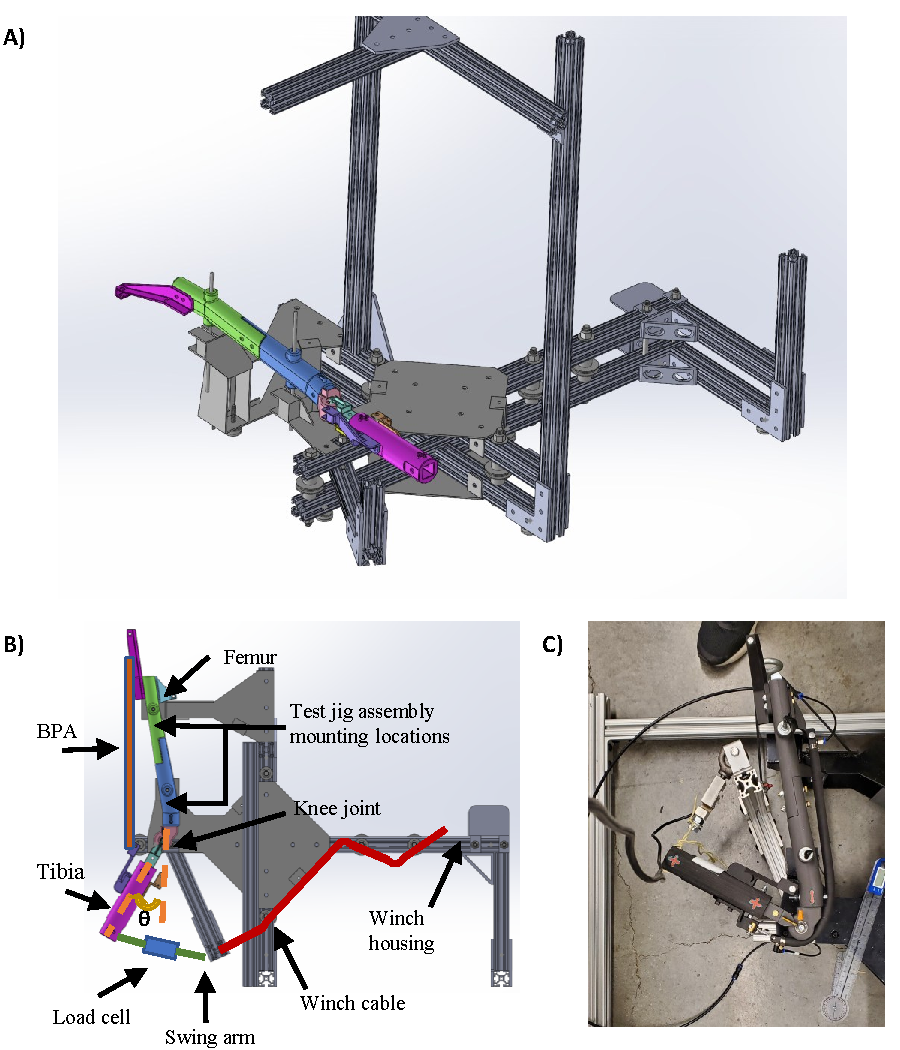
\includegraphics[width=0.9\textwidth]{Figures/testJigs.pdf}
    \end{center}
    \caption{\textbf{(A)} CAD solid model assembly of the revolute joint knee in the test stand. \textbf{(B)} 1-DoF pinned-joint robot knee in the test apparatus with important components labeled; the leg is shown with 30 degrees of flexion, i.e.\ $\theta_{\mathbf{k}} = \ang{-30}$. \textbf{(C)} Picture from isometric torque testing. The setup shows the revolute knee configured for a test of the extensor BPA, with the knee flexed at $\theta_{\mathbf{k}} = \ang{-120}$; note the compressed shape of the inflated BPA on the knee at this high degree of flexion.}\label{fig:testJigs}
\end{figure}

Two knee joints were tested: a pure revolute joint, and a biomimetic joint whose four-bar linkage translates the instantaneous center of rotation (ICR) as the knee rotates \citep{steele_biomimetic_2018,steele_development_2017,steele_biomimetic_2018-1}, moving it posteriorly in $X$ and distally in $Y$ in the femur frame, except briefly proximally near full flexion, much as the human knee does \citep{bolen_determination_2019}. Reference coordinate frames follow \citet{wu_for_1995,wu_isb_2002}, and Figure~\ref{fig:ICR} shows the measured ICR migration. Both joints share the same rotation center in the femur frame at $\theta_{\mathbf{k}} = \ang{0}$, each was driven by an antagonistic flexor and extensor, and $\theta_{\mathbf{k}}$ is negative in flexion throughout this work.

\begin{figure}[htbp]
    \begin{center}
    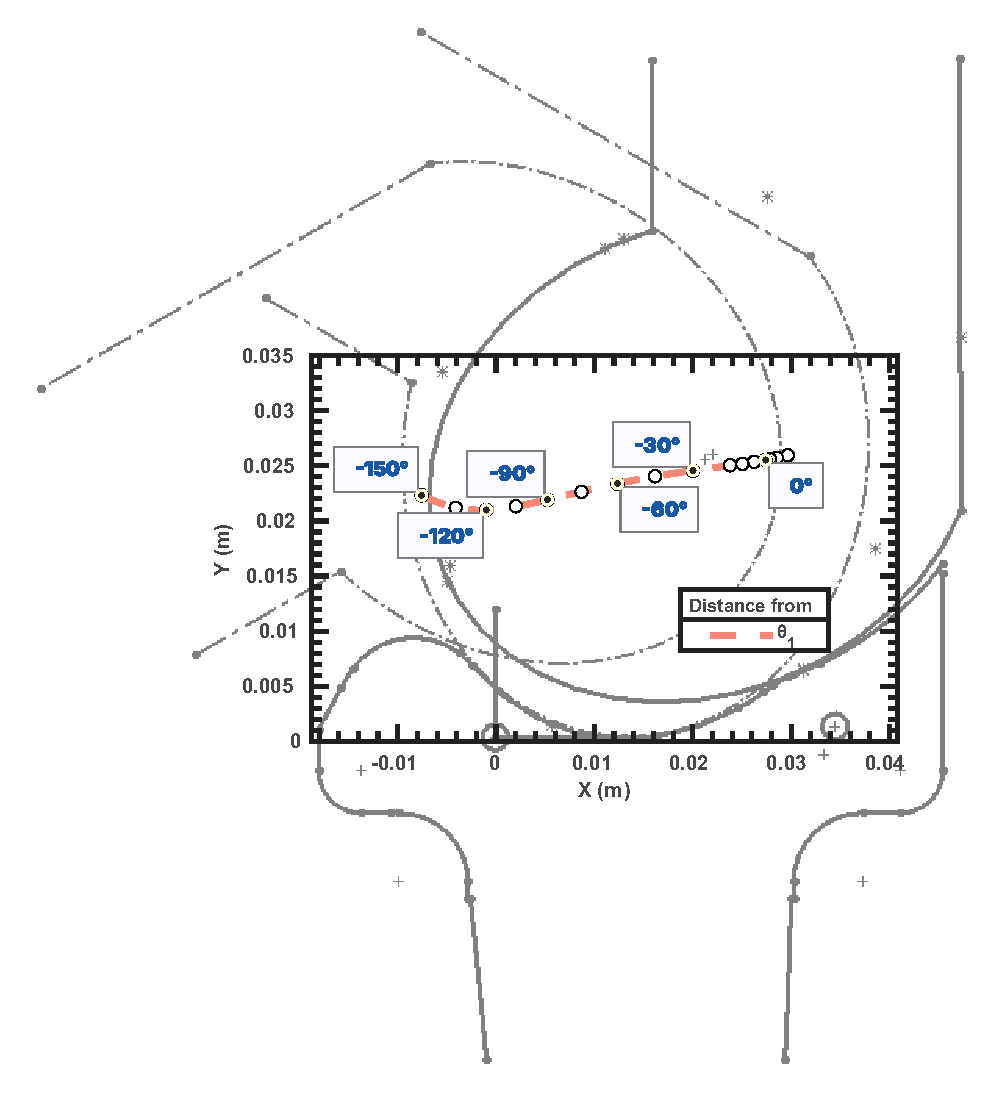
\includegraphics[width=0.8\textwidth]{Figures/KneeICR.eps}
    \end{center}
    \caption{ICR for the biomimetic robot knee as a function of knee angle, measured from $\theta_{1}$ on the tibia. The plot is overlaid on a model of the knee at $\theta_{\mathbf{k}}=0^\circ$ (solid line) and $-60^\circ$ and $-120^\circ$ (dotted dash lines). White circles represent measured points in $-15^\circ$ increments from $-150^\circ$ to $-15^\circ$, in $-5^\circ$ increments from $-15^\circ$ to $0^\circ$, and then at $2^\circ$, $5^\circ$, and $10^\circ$.}\label{fig:ICR}
\end{figure}

Each stand was tested with $\diameter$\qty{10}{\mm} Festo BPAs in both configurations, and the biomimetic knee also with a $\diameter$\qty{20}{\mm} BPA. Each actuator was pinned at its origin on the femur, with the far end either pinned at the tibial insertion or attached there through an artificial tendon. \citet{bolen_determination_2019,morrow_optimization_2020} give full details of the modeled robot and its torque calculation.

\subsection{Equipment and Data Collection}\label{sec:torque_equipment}

A test jig was built to collect knee torque at set knee angles over the range of motion. The stand frame is made of 80/20 1515 series extruded aluminum. The femur is fixed to the frame while the knee rotates the tibia, with the joint axis co-axial with gravity to eliminate gravitational torque. A force sensor connects the tibia to a swing arm tied to a winch with 3/16-inch Kevlar rope (Quality Nylon Rope) routed over idler pulleys. At each measured $\theta_{\mathbf{k}}$ the winch was locked and the BPA was inflated and then deflated, keeping the measurement as isometric as possible. Because the sensor and its rope load path tie the tibia to the locked winch, the sensor reading is the tension that holds the tibia at the set angle. The measured knee torque at each angle is that tension multiplied by the perpendicular distance from the knee axis to the rope's line of action at its tibial attachment, the measured counterpart of the scalar reduction of Equation~\eqref{eq:M_scalar}, with the attachment geometry and the sensor-line angle recorded at each test position.

Force was collected with one of two sensors: a MODERN STEP \qty{300}{\kilo\gram} digital crane scale, or a CALT DYLY-103 \qty{100}{\kilo\gram} S-shaped load cell used with an HX711 load-cell amplifier. Pressure was measured with a Freescale MPX5700 GP \qty{5}{\volt} pressure sensor. Supply pressure was controlled by two regulators in series, a Parker 20R113GC (\qtyrange{0}{120}{\psi}) and a Husky HDA72200, and air was delivered through a Festo VTUG-10 valve manifold. Pressure and load-cell data were sent to MATLAB through a Sparkfun BlackBoard C (Arduino Uno style) microcontroller. Lengths were measured with a tape measure, with a flexible string marking the axial length of the BPA when its curvature was sufficient, and angles with a Medigauge digital goniometer or MALENOO analog goniometers of \qtylist{6;8;12}{\inch} lengths.

\subsection{Hybrid Torque Calculation}\label{sec:hybrid_method}

Torque about the knee is the moment of the actuator force about the ICR. Two vectors enter it: the position vector $\mathbf{d}$ from the ICR to the point of force application, and the force vector $\mathbf{F} = \norm{\mathbf{F}}\hat{\mathbf{u}}$ along the line of action. The signed knee-axis torque is $M_{\mathbf{k}}=\hat{\mathbf{z}}_{\mathbf{k}}\cdot(\mathbf{d}\times\mathbf{F})$. For force acting in the plane normal to the knee axis, the moment-arm magnitude is
\begin{equation}
    r = \norm{\mathbf{d} \times \hat{\mathbf{u}}}
    \label{eq:momentarm_def}
\end{equation}
a scalar distance computed from the vectors or measured directly. For an out-of-plane force, knee torque uses the axis projection above rather than the magnitude of the three-dimensional moment. In the model, the projected moment arm follows the projection method of \citet{young_analyzing_2019}: the scalar moment arm about the joint axis $\hat{\mathbf{z}}_{\mathbf{k}}$ (the knee-frame $Z$ axis) is
\begin{equation}
    r_{\mathbf{k}} = \mathbf{p}_{proj,xy} \cdot \frac{\mathbf{p}_{f} \times \hat{\mathbf{z}}_{\mathbf{k}}} {\norm{\mathbf{p}_{f} \times \hat{\mathbf{z}}_{\mathbf{k}}}} \label{eq:project_ma}
\end{equation}
where $\mathbf{p}_{f}$ is the three-dimensional free muscle segment vector, the segment whose endpoints ride on different bodies and whose in-plane component sets the line of action, and $\mathbf{p}_{proj,xy}$ is the position vector from the joint-axis origin to the point of force application, projected onto the plane normal to the joint axis. The ratio term is the in-plane unit normal to the projected line of action, so the product is the perpendicular distance of Equation~\eqref{eq:momentarm_def}, computed in the tibial body frame.

The hybrid torque calculation localizes disagreement between the model and the measurements. The classical moment is the cross product
\begin{equation}
    \mathbf{M} = \mathbf{d} \times \mathbf{F} \label{eq:M_vec}
\end{equation}
and its scalar component about the joint axis, written $M_{z}$, reduces through the moment arm to the ordinary product
\begin{equation}
    M_{z} = r\,F \label{eq:M_scalar}
\end{equation}
The hybrid method replaces the model-predicted moment arm of Equation~\eqref{eq:project_ma} and the model-predicted muscle length with measured counterparts: $r$ is measured directly as the perpendicular distance from the knee axis to the line of action, and $F$ follows from the measured $P$, $l_{0}$, $l_{620}$, and $l_\text{m}$ through the force model of Section~\ref{sec:force_model}, which separates kinematic error from force error. This calculation is also referred to as the back-calculated torque; the two names denote the same quantity and are used interchangeably in this paper.

\subsection{Improved Torque Model: Length Offset and Bracket Compliance}\label{sec:improved_model}

Measured muscle lengths were consistently shorter than predicted at all joint angles, and the shortfall persisted at $\varepsilon^{*} = 1$ with $F = 0$, indicating a constant rather than a load-dependent offset. The corrected muscle length is therefore
\begin{equation}
    l_\text{m} = l_{LMT} - 2\;l_{fitting} - \chi_{0}
    \label{eq:Lm}
\end{equation}
where $l_{LMT}$ is the musculotendon path length from origin to insertion, $l_{fitting}$ is the end-cap length (\qty{25.4}{\mm} per end), and $\chi_{0}$ is the constant length offset.

As the actuator develops force, the compliant attachments deform, changing the effective BPA length and, through it, the force. The combined compliance is modeled with Hooke's law in a local bracket frame at each attachment. The two-rotation frame is constructed from the vector joining the bracket reference point to the BPA attachment point, $\mathbf{p}_{A}$ at the femur-side muscle origin or $\mathbf{p}_{B}$ at the tibial insertion (Figure~\ref{fig:xiFrameTransform}): a rotation through $\theta_z$ about the fixed space-frame axis $\hat{\mathbf{z}}_{s}$ aligns an intermediate axis with the sagittal-plane projection of the attachment point, and a rotation through $-\theta_y$ about the current $\hat{\mathbf{y}}$ axis, which points posteriorly in the primary cantilever bending direction, aligns the bracket axis $\hat{\mathbf{x}}_{br}$ with the full three-dimensional point vector. The orientation and homogeneous transform are
\begin{equation}
\mathbf{R}_{sb}=\mathbf{R}_z(\theta_z)\mathbf{R}_y(\theta_y)^T.
\label{eq:bracket_frame_rotation}
\end{equation}
\begin{equation}
\mathbf{T}_{sb}=
\begin{bmatrix}
\mathbf{R}_{sb} & \mathbf{p}_{br}\\
\mathbf{0}^{T} & 1
\end{bmatrix}.
\label{eq:bracket_frame_transform}
\end{equation}
Figure~\ref{fig:bktFrame} shows the bracket frame for each test configuration.



\begin{figure}[htbp]
\begin{center}
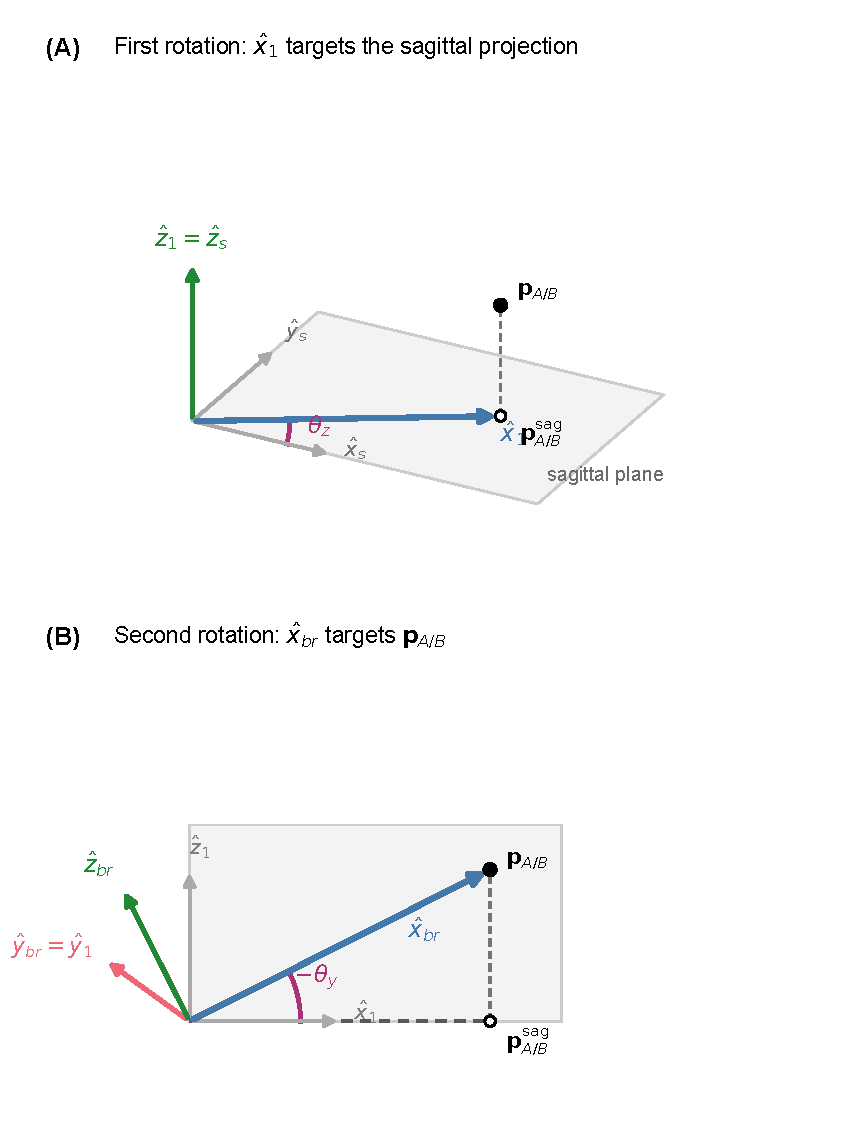
\includegraphics[height=0.62\textheight]{Figures/xiFrameTransform.pdf}
\end{center}
\caption{Two-rotation construction of the bracket frame from the attachment point $\mathbf{p}_{A}$, the femur-side muscle origin, or $\mathbf{p}_{B}$, the tibial insertion. \textbf{(A)} Rotation through $\theta_z$ about the fixed $\hat{\mathbf{z}}_{s}$ axis aligns the intermediate axis $\hat{\mathbf{x}}_{1}$ with the point's sagittal-plane projection. \textbf{(B)} Rotation through $-\theta_y$ about the current $\hat{\mathbf{y}}_{1}=\hat{\mathbf{y}}_{br}$ axis aligns the final bracket axis $\hat{\mathbf{x}}_{br}$ with the full point vector.}\label{fig:xiFrameTransform}
\end{figure}

\begin{figure}[htbp]
\begin{center}
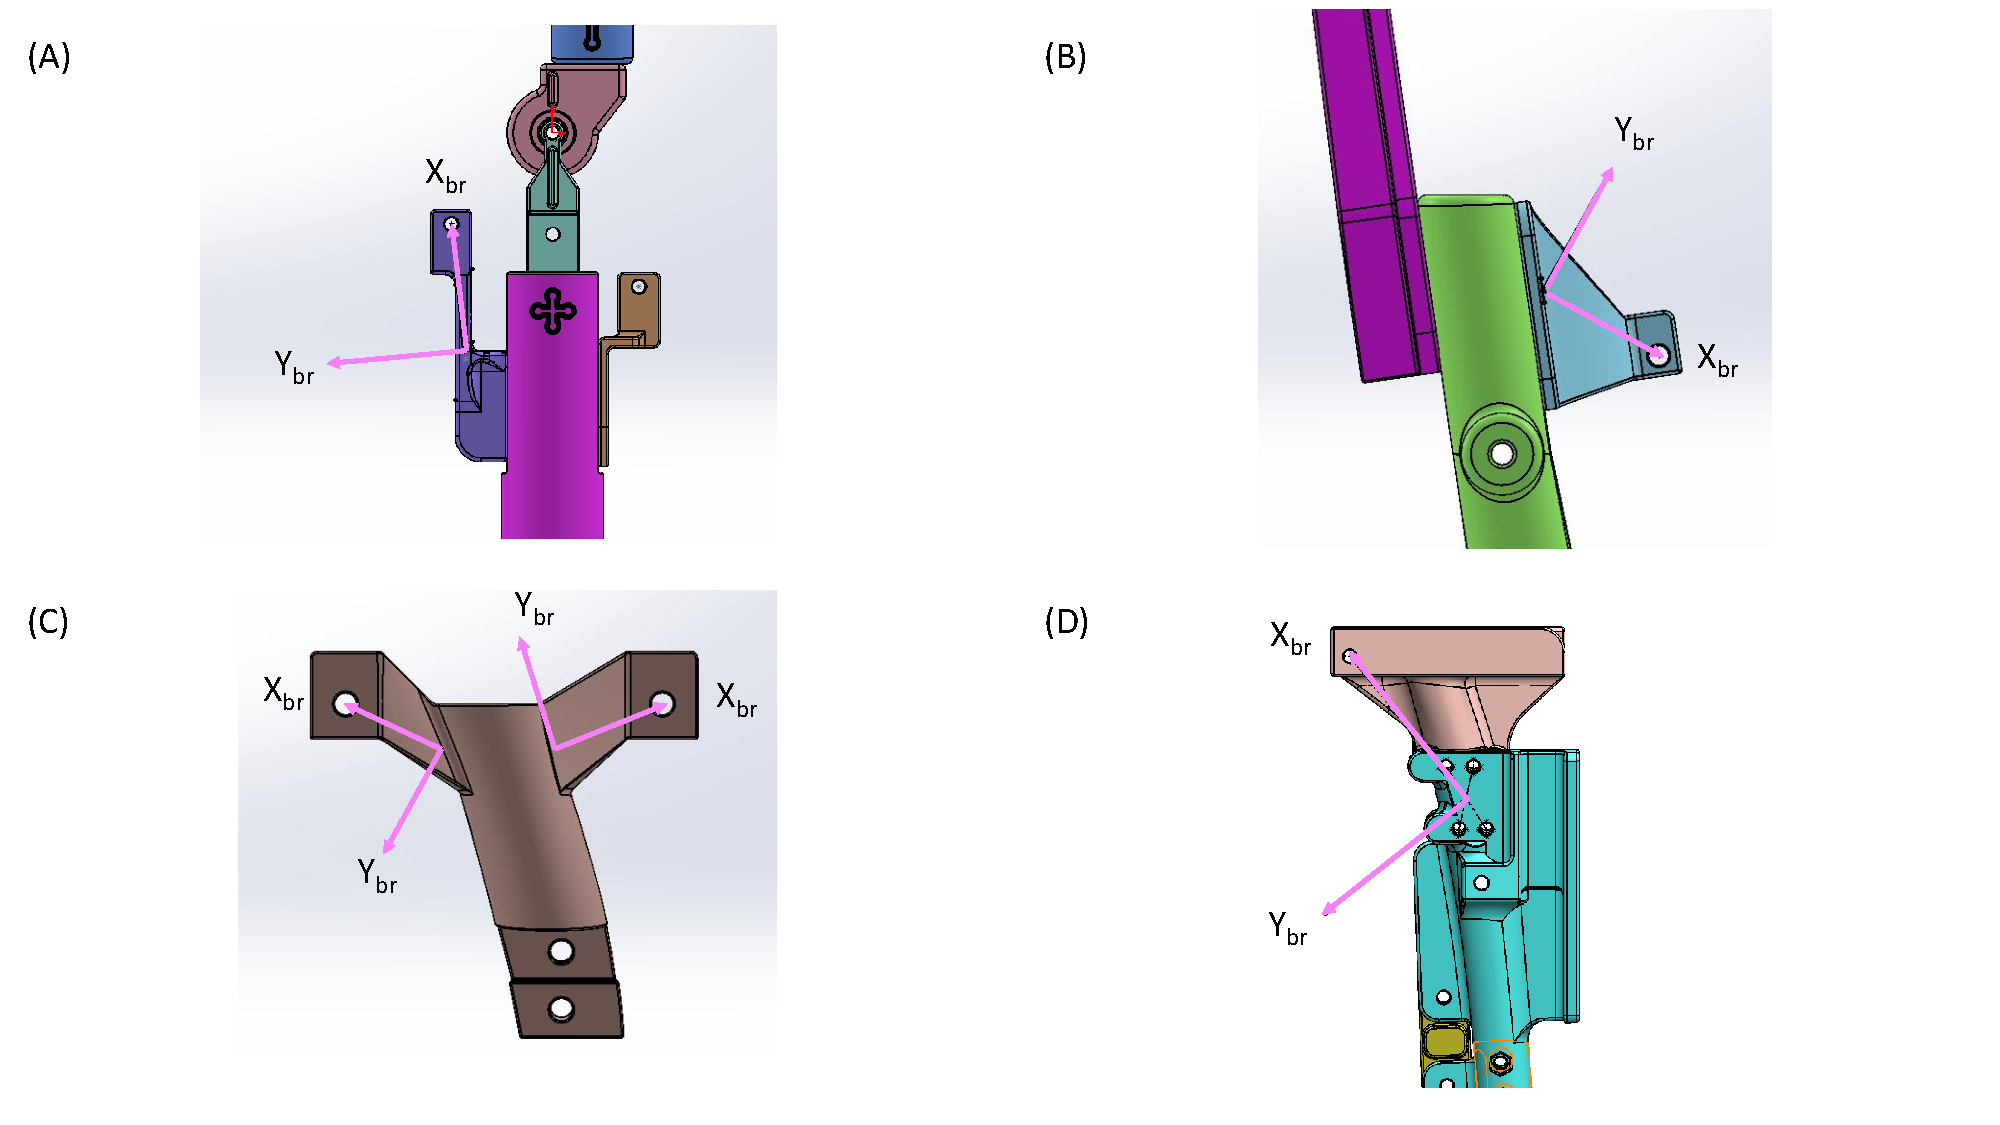
\includegraphics[width=1\textwidth]{Figures/bktFrame.pdf}
\end{center}
\caption{Bracket frame orientations for: \textbf{(A)} flexor configuration on the pinned knee, \textbf{(B)} extensor configuration on the pinned knee, \textbf{(C)} flexor and extensor configurations on the biomimetic knee with $\diameter$\qty{10}{\mm} BPAs, and \textbf{(D)} flexor configuration on the biomimetic knee with the $\diameter$\qty{20}{\mm} BPA.}\label{fig:bktFrame}
\end{figure}

In each local frame the bracket is modeled as three independent linear springs. For the pinned-flexor insertion bracket, the identified stiffness assignment is
\begin{equation}
\mathbf{K}_{br} =
\begin{bmatrix}
\chi_{1} & 0   & 0 \\
0   & \chi_{2} & 0 \\
0   & 0   & \chi_{1} \\
\end{bmatrix}
\label{eq:bktstiffness}
\end{equation}
with $\chi_{1}$ assigned to $x_{br}$ and $z_{br}$, and $\chi_{2}$ to $y_{br}$. The stiffness pair is shared across configurations, but its axis assignment follows the hardware model: the pinned-flexor origin bracket uses $\operatorname{diag}(\chi_1,\chi_1,\chi_2)$, the pinned extensor and biomimetic flexor use $\operatorname{diag}(\chi_1,\chi_2,\chi_2)$, and the biomimetic extensor uses Equation~\eqref{eq:bktstiffness}. The adopted two-bracket flexor fit and pinned-extensor fit use the two-rotation construction. A rotation about $y_{br}$ leaves a stiffness matrix unchanged only when its $x_{br}$ and $z_{br}$ stiffnesses are equal. Frame independence therefore applies to Equation~\eqref{eq:bktstiffness}, not to every assignment.

The local force vector is the force magnitude times its unit direction,
\begin{equation}
\mathbf{F}_{br}=F\hat{\mathbf{u}}.
\label{eq:bktforcevector}
\end{equation}
where $\hat{\mathbf{u}}=[u_x,u_y,u_z]^T$ is the local unit force direction.
Hooke's law relates this force to the bracket displacement vector:
\begin{equation}
\mathbf{F}_{br}=\mathbf{K}_{br}\boldsymbol{\eta}_{br}.
\label{eq:bktforcebalance}
\end{equation}
\begin{equation}
\mathbf{C}_{br}=\mathbf{K}_{br}^{-1}.
\label{eq:bktcompliance}
\end{equation}
\begin{equation}
\boldsymbol{\eta}_{br}=\mathbf{C}_{br}\mathbf{F}_{br}.
\label{eq:bktdeflection}
\end{equation}
For the insertion-bracket assignment of Equation~\eqref{eq:bktstiffness}, this gives
\begin{equation}
\boldsymbol{\eta}_{br}=F
\begin{bmatrix}u_x/\chi_1\\u_y/\chi_2\\u_z/\chi_1\end{bmatrix}.
\label{eq:bktcomponentdeflection}
\end{equation}
The displacement need not be parallel to the force. Only its projection along the local line of action contributes to the scalar shortening used in the force balance (Figure~\ref{fig:xiProjection}):
\begin{equation}
\delta_{br}=\hat{\mathbf{u}}^T\boldsymbol{\eta}_{br}.
\label{eq:bktprojecteddeflection}
\end{equation}
Substitution of Equation~\eqref{eq:bktdeflection} gives
\begin{equation}
\delta_{br} = F\, \hat{\mathbf{u}}^{T} \, \mathbf{K}_{br}^{-1} \, \hat{\mathbf{u}}
\label{eq:bktprojectedcompliance}
\end{equation}
so the projected bracket compliance is
\begin{equation}
c_{\hat{u},br} = \frac{\delta_{br}}{F} = \hat{\mathbf{u}}^{T} \mathbf{C}_{br} \hat{\mathbf{u}}
\label{eq:keff}
\end{equation}
along the force path. An artificial tendon is modeled as an axial spring of stiffness $k_{ten} = n A_{c} E / L_{ten}$, with $n = 2$ parallel cable strands (six for the $\diameter$\qty{20}{\mm} assembly), effective metallic cross-sectional area of the stranded cable $A_{c} = \qty{1.51e-6}{\metre\squared}$, and modulus $E = \qty{193}{\giga\pascal}$. Bracket deflection and tendon stretch both shorten the effective BPA length under the same force, so their scalar compliances add in series:
\begin{equation} c_{eq} = c_{\hat{u},br} + c_{ten}
\label{eq:equivalentstiffness}
\end{equation}

The tendon compliance is $c_{ten}=k_{ten}^{-1}$, and the equivalent stiffness is $k_{eq}=c_{eq}^{-1}$. This reduction assumes quasi-static tensile loading, linear translational springs, and additive displacements along the force path. The direction is held fixed during the scalar solve, then updated with the displaced attachments; rotational compliance and force--moment coupling are not modeled. With a second compliant bracket, the same reduction gives
\begin{equation}
k_{eq}^{-1}=\sum_j\hat{\mathbf{u}}_j^T\mathbf{K}_{br,j}^{-1}\hat{\mathbf{u}}_j+k_{ten}^{-1},
\label{eq:two_bracket_stiffness}
\end{equation}
where the tendon term is omitted for a direct attachment. All unit directions and stiffness matrices in a projection are expressed in the same local frame.

The compliance displacement shortens the actuator, so the active length entering the force model is
\begin{equation} l_m(\delta) = l_m^{(0)} - \delta
\label{eq:activelengthcorrected}
\end{equation}
where $l_m^{(0)}$ is actuator length before displacement. Because the force depends on contraction, and the contraction on the compliance displacement, $\delta$ is the root of the implicit balance
\begin{equation} F_{620}(l_{0}) \, F^{*}\!\left(\varepsilon^*(\delta),P^*\right) - k_{eq}\,\delta = 0
\label{eq:complianceforcebalance}
\end{equation}
solved by bracketed scalar root-finding between zero deflection and the deflection that would bring the actuator to its maximum usable contraction, with $\delta = 0$ returned when the residual shows no sign change across that interval. The solved force gives the vector bracket deflection, which updates the attachment location; the routed length, force direction, moment arm, and torque are recalculated at the deflected geometry. The stiffness terms are effective parameters for the attachment system as a whole, absorbing the printed brackets, the bone fixtures, and the winch cable, and they are identified from torque rather than measured on any component in isolation.

Figure~\ref{fig:xiProjection} shows how both ends of the actuator path can be compliant: the insertion-side bracket together with a second, origin-side bracket. Each bracket $j$ develops a three-dimensional deflection $\boldsymbol{\eta}_{br,j}$ along its local frame basis, of which only the projection along the corresponding force direction $\hat{\mathbf{u}}_j$ changes the actuator length, and the two projections act in series with the tendon elongation:
\begin{equation}
\begin{aligned}
\boldsymbol{\eta}_{br,j} &= \sum_{i=1}^{3}\eta_{i,j}\hat{\mathbf{e}}_i^{(j)},\\
\delta_{br,j} &= \hat{\mathbf{u}}_j^T\boldsymbol{\eta}_{br,j}, \qquad j\in\{1,2\},\\
\delta_{\mathrm{series}} &= \delta_{br,1}+\delta_{\mathrm{tendon}}+\delta_{br,2}.
\end{aligned}
\label{eq:bracket_series_projection}
\end{equation}

\begin{figure}[htbp]
\centering
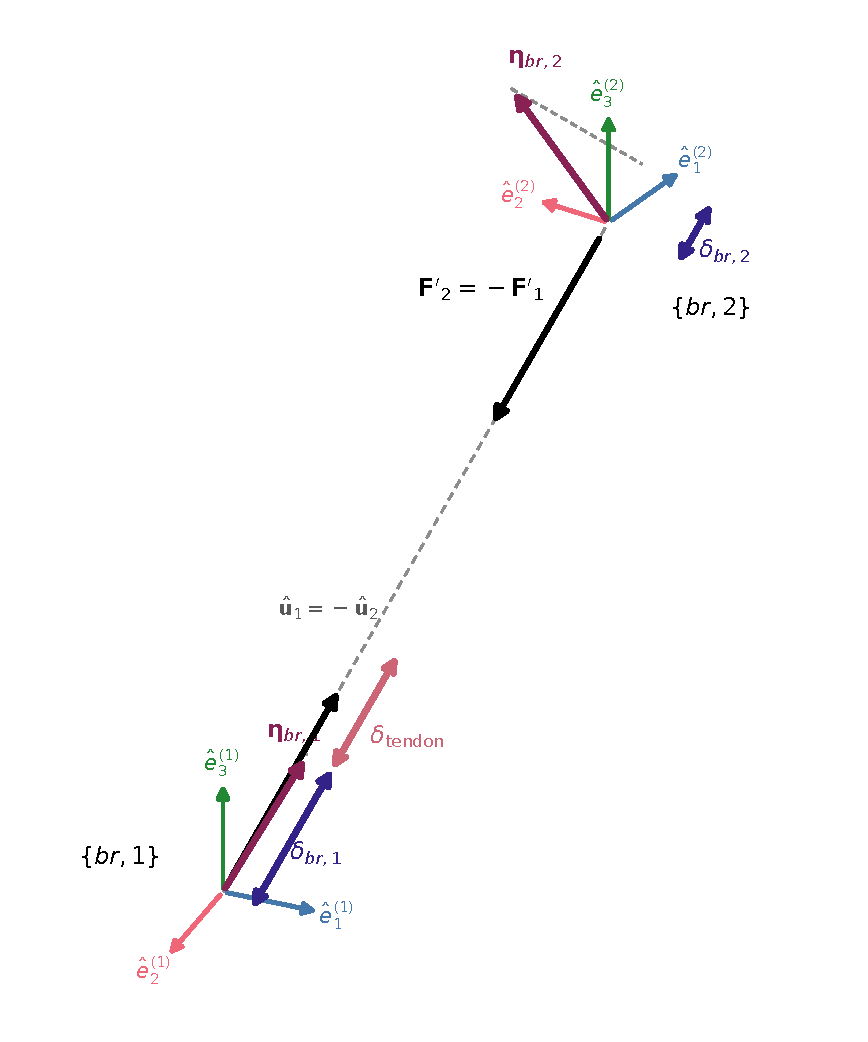
\includegraphics[width=0.65\textwidth,height=0.58\textheight,keepaspectratio]{Figures/xiProjection.pdf}
\caption{Projection of bracket displacement onto the actuator force path. Each bracket has a local basis $\hat{\mathbf e}^{(j)}_1$, $\hat{\mathbf e}^{(j)}_2$, and $\hat{\mathbf e}^{(j)}_3$. The displacement $\boldsymbol\eta_{br,j}$ has an axial projection $\delta_{br,j}$ along $\hat{\mathbf u}_j$; the two bracket projections and tendon elongation contribute to the change in actuator length. Displacements are exaggerated.}
\label{fig:xiProjection}
\end{figure}

\subsection{Fictive Strain and Wrapping Loss}\label{sec:fictive_contraction}

As the knee flexes, the extensor BPA contacts the anterior joint surface and bends around it (Figure~\ref{fig:bpaWrapping}). The rigid routed-length calculation does not account for the resulting change in usable contraction. We represent this effect with fictive strain: an empirical increase in the contraction seen by the force model, beyond the actuator's geometric contraction. The correction is phenomenological; it does not resolve wall stresses or the deformation of the braided actuator. A wrapping-loss term $\chi_3$ scales the associated reduction in usable length:
\begin{equation}
    \Delta l = \begin{cases}
     \chi_{3}\;R\;\abs{ \theta_\text{wrap}-\theta_{\mathbf{k}}}\;\zeta^2 & \theta_{\mathbf{k}} \leq      \theta_\text{wrap} \\
      0 & \theta_{\mathbf{k}} \geq      \theta_\text{wrap}
     \end{cases}\label{eq:deltaL}
\end{equation}
where $\Delta l$ is the change in usable length of the BPA, $R$ is the wrapping radius, $\abs{\theta_\text{wrap}-\theta_{\mathbf{k}}}$ is the angle through which the BPA is bent once contact begins, and $\theta_\text{wrap}$, the knee flexion angle at which the BPA starts to bend over the joint, is determined from solid modeling. The factor $\zeta$ is the additive complement to the relative contraction,
\begin{equation}
    \zeta = 1-\varepsilon^*
\label{eq:comp}
\end{equation}
so the wrapping loss vanishes at full contraction and grows quadratically toward resting length. Combining Equations~\eqref{eq:comp} and~\eqref{eq:deltaL} with the offset of Equation~\eqref{eq:Lm} yields the fully corrected muscle length
\begin{equation}
    l_\text{m} = l_{LMT} - 2\;l_{fitting}  - \chi_{0} - \Delta l\label{eq:x3}
\end{equation}
 
\begin{figure}[H]
\centering
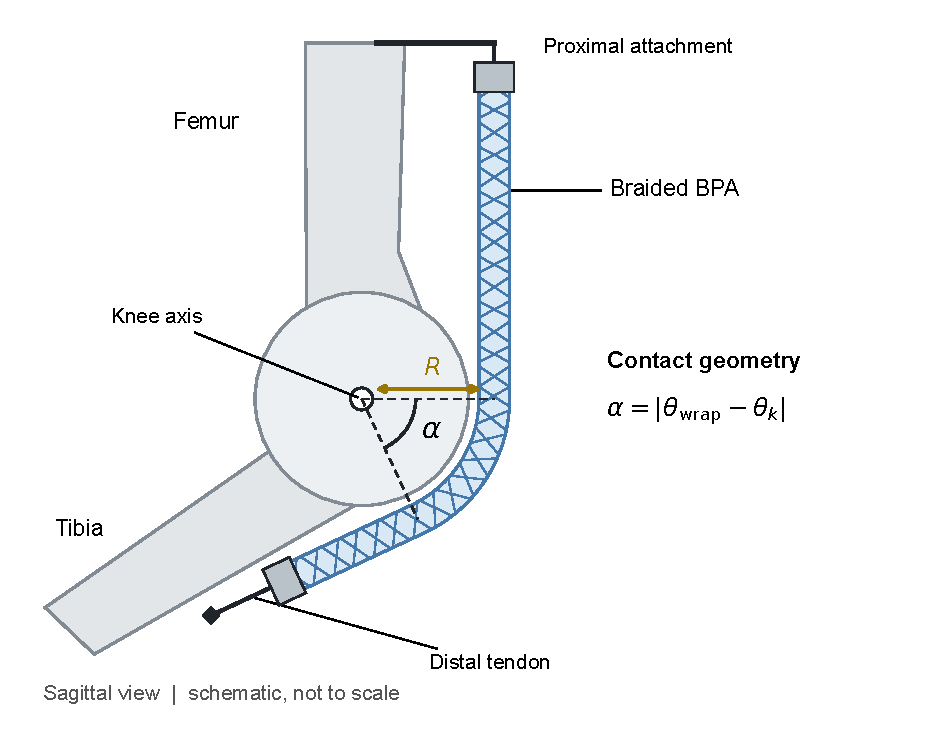
\includegraphics[width=0.75\textwidth]{Figures/bpa_knee_wrapping_review.pdf}
\caption[BPA crossing a flexed knee]{Sagittal schematic of an extensor BPA crossing a flexed robot knee, with its braided body following an anterior contact arc between the proximal attachment and distal tendon. Dashed radii bound the contact arc; $R$ is the BPA-path wrapping radius, and $\alpha=\abs{\theta_{\mathrm{wrap}}-\theta_{\mathbf{k}}}$ is the bend angle after contact begins, expressed in radians in Equation~\eqref{eq:deltaL}. The drawing illustrates the local circular-wrap approximation, not the full multi-contact route. The fitted usable-length loss $\Delta l$ is not an arc-minus-chord length.}
\label{fig:bpaWrapping}
\end{figure}

\subsection{Identification Procedure}\label{sec:identification}

The correction terms were identified by global optimization against measured isometric torque. For a candidate correction vector $\boldsymbol{\chi}$, $(\chi_{0}, \chi_{1}, \chi_{2})$ in the flexor stage and $(\chi_{0}, \chi_{3})$ on the locked stiffness pair in the extensor refit, the predicted torque curve of test $i$ is interpolated to its $n_{i}$ measured knee angles $\theta_{ij}$, giving residuals $e_{ij} = M_{ij} - \hat{M}(\theta_{ij}; \boldsymbol{\chi})$ against the measured torque $M_{ij}$, and the three goodness-of-fit (GoF) components of that test are
\begin{equation}
\mathrm{RMSE}_{i} = \sqrt{\frac{1}{n_{i}}\sum_{j} e_{ij}^{2}}\label{eq:gof_components}
\end{equation}
\begin{equation}
\mathrm{FVU}_{i} = \frac{n_{i}-1}{n_{i}} \cdot \frac{\sum_{j} e_{ij}^{2}}{\sum_{j} (M_{ij} - \bar{M}_{i})^{2}}\label{eq:gof_fvu}
\end{equation}
\begin{equation}
e^{\max}_{i} = \max_{j} \abs{e_{ij}}.\label{eq:gof_max}
\end{equation}
RMSE summarizes the overall error magnitude. FVU expresses the residual sum of squares relative to the sum of squared deviations of the measured torque from its mean $\bar{M}_{i}$, with the factor $(n_{i}-1)/n_{i}$ carrying the small-sample adjustment of the evaluators. The maximum absolute residual records the largest pointwise error. RMSE and the maximum residual have torque units, whereas FVU is dimensionless; smaller values indicate closer agreement for all three. The solver minimizes the objective vector
\begin{equation}
\mathbf{g}(\boldsymbol{\chi}) = \frac{1}{\abs{\mathcal{T}}} \sum_{i \in \mathcal{T}}
\begin{bmatrix}
g_{1,i}(\boldsymbol{\chi})/g_{1,i}^{(0)} \\
g_{2,i}(\boldsymbol{\chi})/g_{2,i}^{(0)} \\
g_{3,i}(\boldsymbol{\chi})/g_{3,i}^{(0)}
\end{bmatrix},
\label{eq:gof_objective}
\end{equation}
where $g_{1,i}$, $g_{2,i}$, and $g_{3,i}$ are the RMSE, FVU, and maximum absolute residual of Equations~\eqref{eq:gof_components}--\eqref{eq:gof_max}, the superscript $(0)$ marks the zero-correction baseline value of the same component, with the correction terms disabled, and $\mathcal{T}$ is the set of tests used for training; the mean of the baseline-normalized components makes the three objectives dimensionless and the training tests commensurate. The search carried no constraints beyond the parameter bounds of each stage, and the returned Pareto fronts were filtered to members scoring at or below the zero-correction baseline on every component of every test in that stage's identification pool.

Together, these measures assess agreement in torque magnitude and variation across the range of motion. Offsets, amplitude differences, and shifts along the knee-angle axis can affect several metrics at once, so the metrics are interpreted jointly rather than assigning each one to a single type of disagreement. Across tests with different torque ranges, the absolute and variance-normalized errors also weight the tests differently. Multiobjective optimization retains these comparisons alongside the largest local error, making the trade-offs visible instead of allowing a favorable average score to conceal a poor fit elsewhere. The resulting Pareto front contains alternative compromises among the objectives, from which the adopted terms are selected using held-out validation.

The solver was MATLAB's elitist nondominated-sorting genetic algorithm, \texttt{gamultiobj} (RRID:SCR\_001622), with adaptive-feasible mutation, scattered crossover at a fraction of 0.8, and a Pareto fraction of 0.35. Candidate terms were evaluated on training and validation tests, and the adopted flexor and extensor solutions share one effective stiffness pair.

The identification proceeded in two stages. The flexor stage fits the two-bracket model $(\chi_{0}, \chi_{1}, \chi_{2})$ across the four pinned-knee flexor tests, with the $l_{0}=\qty{48.5}{\cm}$ and \qty{41.0}{\cm} tests in training and the $l_{0}=\qty{45.7}{\cm}$ and \qty{40.6}{\cm} tendon tests held out for validation. It evolved a population of 150 for up to 600 generations, terminating early once the relative change in the spread of the Pareto front fell below $4\times10^{-3}$. The extensor stage locks $(\chi_{1}, \chi_{2})$ to a member of the flexor Pareto front, enforcing a single stiffness pair across configurations, and solves only the extensor-specific terms $(\chi_{0}, \chi_{3})$ on a six-test pool of the pinned-extensor campaign, at resting lengths of \qty{40.0}{\cm} plain and with tendon, \qty{43.6}{\cm}, \qty{43.2}{\cm} with tendon, \qty{45.7}{\cm}, and \qty{46.5}{\cm}, with the \qty{43.6}{\cm}, \qty{43.2}{\cm}-tendon, and \qty{45.7}{\cm} tests in training and the \qty{40.0}{\cm} plain, \qty{40.0}{\cm}-tendon, and \qty{46.5}{\cm} tests held out for validation, and the extensor offset allowed negative values. The refit used a population of 50 for up to 150 generations at a spread tolerance of $1\times10^{-3}$. Both stages searched a normalized space, with length offsets in centimeters and stiffnesses on a base-ten logarithmic scale, so that the genetic search samples the decade-spanning stiffness bounds uniformly. Expressed in physical units, the flexor bounds were $\chi_{0} \in [0, 20]$~\si{\milli\metre}, $\chi_{1} \in [3\times10^{4}, 10^{6}]$~\si{\N\per\metre}, and $\chi_{2} \in [5\times10^{3}, 2\times10^{4}]$~\si{\N\per\metre}; the extensor refit searched $\chi_{0} \in [-20, +5]$~\si{\milli\metre} and $\chi_{3} \in [0, 1]$ with the stiffness pair locked. The initial flexor population was drawn from $\chi_{0} \in [5, 15]$~\si{\milli\metre}, $\chi_{1} \in [5\times10^{4}, 5\times10^{5}]$, and $\chi_{2} \in [7\times10^{3}, 1.5\times10^{4}]$~\si{\N\per\metre}.

\subsection{Route-Redesign Procedure}\label{sec:route_redesign}

With the correction terms fixed, the attachment routes themselves become design variables, and their best values are the ones that make the redesigned routes meet or exceed human knee torque capability. The redesign was carried out on the robot-body model derived from the Gait2392 lower-extremity model \citep{delp_opensim_2007,seth_opensim_2018}. The human targets are maximum-isometric torque curves: OpenSim moment arms, the partial derivative of muscle-tendon length with respect to the knee coordinate, $r(\theta_{\mathbf{k}}) = \partial l_{\mathrm{MT}}/\partial\theta_{\mathbf{k}}$, multiplied by each muscle's maximum isometric force \citep{delp_interactive_1990,hoy_musculoskeletal_1990,yamaguchi_planar_1989,sherman_what_2013,millard_flexing_2013,thelen_adjustment_2003,seth_opensim_2011}. The extensor is graded against vastus medialis and the flexor against biceps femoris short head; each target includes a 5\,\% torque margin as a design factor for additional effects not represented by the model. The required prediction is therefore 1.05 times the human target at every design angle.

The design variables are the BPA origin $\mathbf{p}_{1}$, the insertion $\mathbf{p}_{\mathrm{end}}$, the resting length, and the tendon length. Because the route prediction (contact activation, wrapping, and the compliance correction) is expensive to evaluate and only moderately smooth, the redesign minimizes a scalar cost assembled from weighted penalty terms:
\begin{equation}
    J = w_{w}\,J_{\text{worst}} + w_{t}\,J_{\text{torque}} + \textstyle\sum_{a} J_{a} + J_{\text{geom}} + J_{\text{len}}
    \label{eq:opt_cost}
\end{equation}
where $J_{\text{worst}}$ is the largest fraction by which robot torque falls short of the human target at any angle, weighted at $w_{w} = 10^{5}$, and $J_{\text{torque}}$ is the mean-squared shortfall fraction, weighted at $w_{t} = 10^{3}$, two orders of magnitude lower so that no single-angle shortfall can be traded for a better average. The $J_{a}$ are configuration-specific penalties (torque overshoot above the human curve, off-axis torque, wrap release), and $J_{\text{geom}}$ and $J_{\text{len}}$ regularize the endpoints and actuator lengths toward their seed values. Hard constraints, including bone clearance, wrap feasibility, actuator strain and contraction limits, and tendon geometry, reject failed candidates with a prohibitive penalty. The shared actuator plan is two $\diameter$\qty{20}{\mm} BPAs per route under a \qty{620}{\kPa} pressure ceiling, with a maximum usable contraction of 0.255 in the force model: the flexor model carries its two actuators on two separately solved routes, the second derived from the first by a mirrored distal attachment, with the two actuator forces summed, and the extensor model scales the force of a single shared route by the actuator count. Adjacent routes are required to maintain \qty{25}{\mm} of clearance.

A surrogate-assisted global search evaluated up to 3,000 candidate extensor designs and 1,000 candidate flexor designs. A derivative-free pattern search then refined the best feasible design for up to 15,000 further evaluations, stopping earlier if its search-step size fell below the specified tolerance with the constraints satisfied. These budgets limit computation rather than establish convergence by themselves.

The contact-release calculation is given in the Supplementary Material (Section~\ref{app:contact_release}). The cam variant additionally varies the tibial routing profile. Pulley variants introduce a force--travel trade-off: a tackle with $G$ moving line parts multiplies insertion travel by $G$ and divides delivered force by $G$. With $n$ parallel BPAs, the force gain relative to one actuator is $n/G$. Thus, three BPAs through a two-part tackle provide 1.5 times the force and twice the travel of a single direct-drive BPA. Actuator and tendon lengths are re-solved for each transmission configuration. Figure~\ref{fig:reverse_pulley_principle} shows these relations and the separate mounting loads.

\begin{figure}[htbp]
\centering
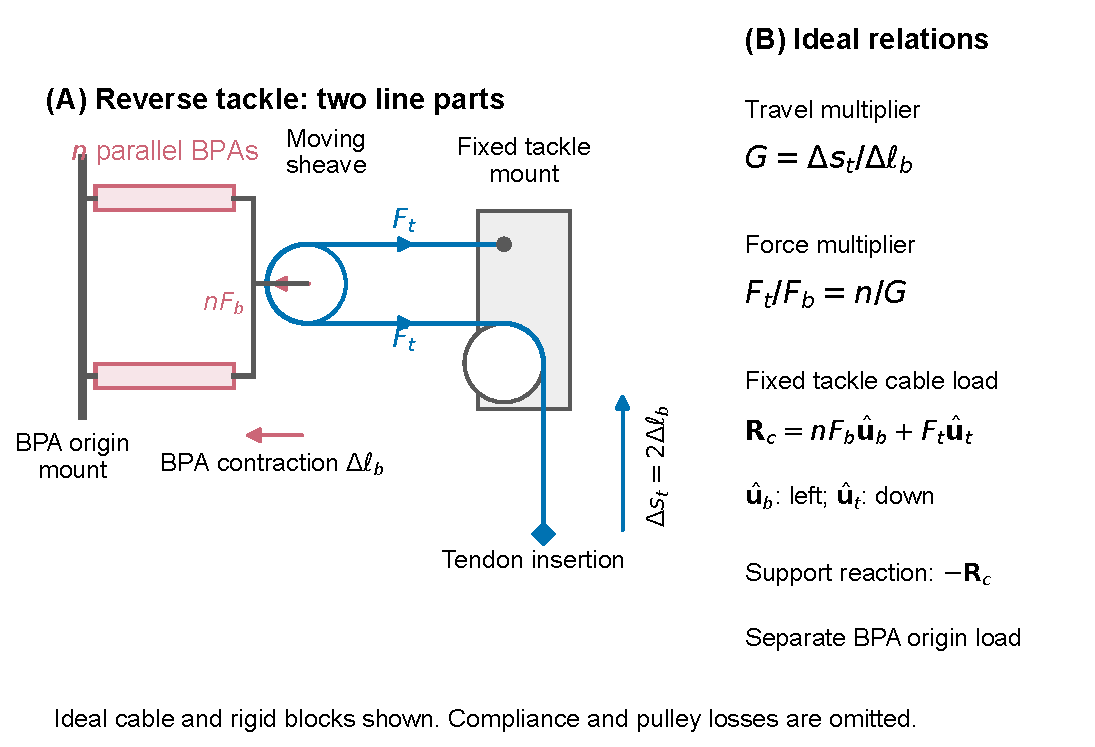
\includegraphics[width=\textwidth]{Figures/reverse_pulley_principle.pdf}
\caption[Reverse-pulley force and travel relations]{Reverse-pulley principle for two moving-block cable parts (A), and ideal force, travel, and mounting-load relations (B). Each of the $n$ parallel BPAs supplies force $F_b$. The travel multiplier is $G$; force gain relative to one BPA is $n/G$. The cable load on the fixed tackle mount combines the forces along the moving-block and insertion-side cable directions. Its support reaction is equal and opposite. The BPA origin mount carries a separate load. Compliance and pulley losses are omitted from this schematic.}
\label{fig:reverse_pulley_principle}
\end{figure}



\section{Results}\label{sec:results_torque}

Measured torque was compared with predictions from the improved BPA force model before and after design-parameter optimization. The pinned-knee flexor tests also compare the original Hunt actuator model with the improved force model. Because the improved model gives closer agreement, the subsequent configurations retain it. Hybrid calculations using measured muscle length and moment arm are shown for the pinned-knee tests to help separate force-model error from geometric error. Those measurements are difficult for a curved BPA near the biomimetic knee's ICR, which lies within the femoral condyles. The biomimetic-extensor hybrid curve in Figure~\ref{fig:Ext10mm_52cm}\textbf{(B)} is therefore treated as an approximate diagnostic rather than an independent validation reference. The training and validation tests are defined in Section~\ref{sec:identification}.

\subsection{Flexor on Pin Joint}

Figure~\ref{fig:FlxPin} compares the measured pinned-knee flexor torque with the pre-correction predictions. Both force models overpredict torque magnitude. On the common domain where both are defined, the improved force characterization gives smaller errors than the Hunt-equation prediction (Supplementary Table~\ref{tab:FlxPinPreGof}). Near full extension the Hunt prediction is undefined, while the improved force model remains defined but has large torque residuals. The hybrid calculation uses measured muscle length and moment arm; its closer agreement identifies an important contribution from the predicted geometry.

The flexor identification of record is the two-bracket fit of Section~\ref{sec:identification} on the four cross-validation tests: the $l_{0}=\qty{48.5}{\cm}$ and \qty{41.0}{\cm} tests in training and the $l_{0}=\qty{45.7}{\cm}$ and \qty{40.6}{\cm}-tendon tests held out. Its adopted design parameters are a length offset $\chi_{0} = \qty{+3.94}{\mm}$ and attachment stiffness parameters $\chi_{1} = \qty{39.98}{\kilo\newton\per\meter}$ and $\chi_{2} = \qty{14.73}{\kilo\newton\per\meter}$ (Table~\ref{tab:AdoptedXi}). Figure~\ref{fig:FlxPin_optimized} shows that, at these terms, the optimized model follows the measured torque across the range of motion, including the loss of torque near full extension that the rigid-body prediction does not produce. The training-set RMSE is \qty{2.165}{\newton\meter} for the $l_{0}=\qty{48.5}{\cm}$ test and \qty{1.084}{\newton\meter} for the $l_{0}=\qty{41.0}{\cm}$ test, and the held-out validation tests give \qty{1.368}{\newton\meter} at \qty{45.7}{\cm} and \qty{1.611}{\newton\meter} at \qty{40.6}{\cm} with tendon (Table~\ref{tab:FlxPinGof}).

The two model predictions in Supplementary Table~\ref{tab:FlxPinPreGof} use their common defined domain: 75 of 90, 17 of 20, 14 of 19, and 15 of 22 measured points in A--D, respectively. The hybrid calculation uses all measured points. Table~\ref{tab:FlxPinGof} reports the full-test errors after correction.

\begin{figure}[htbp]
\begin{center}
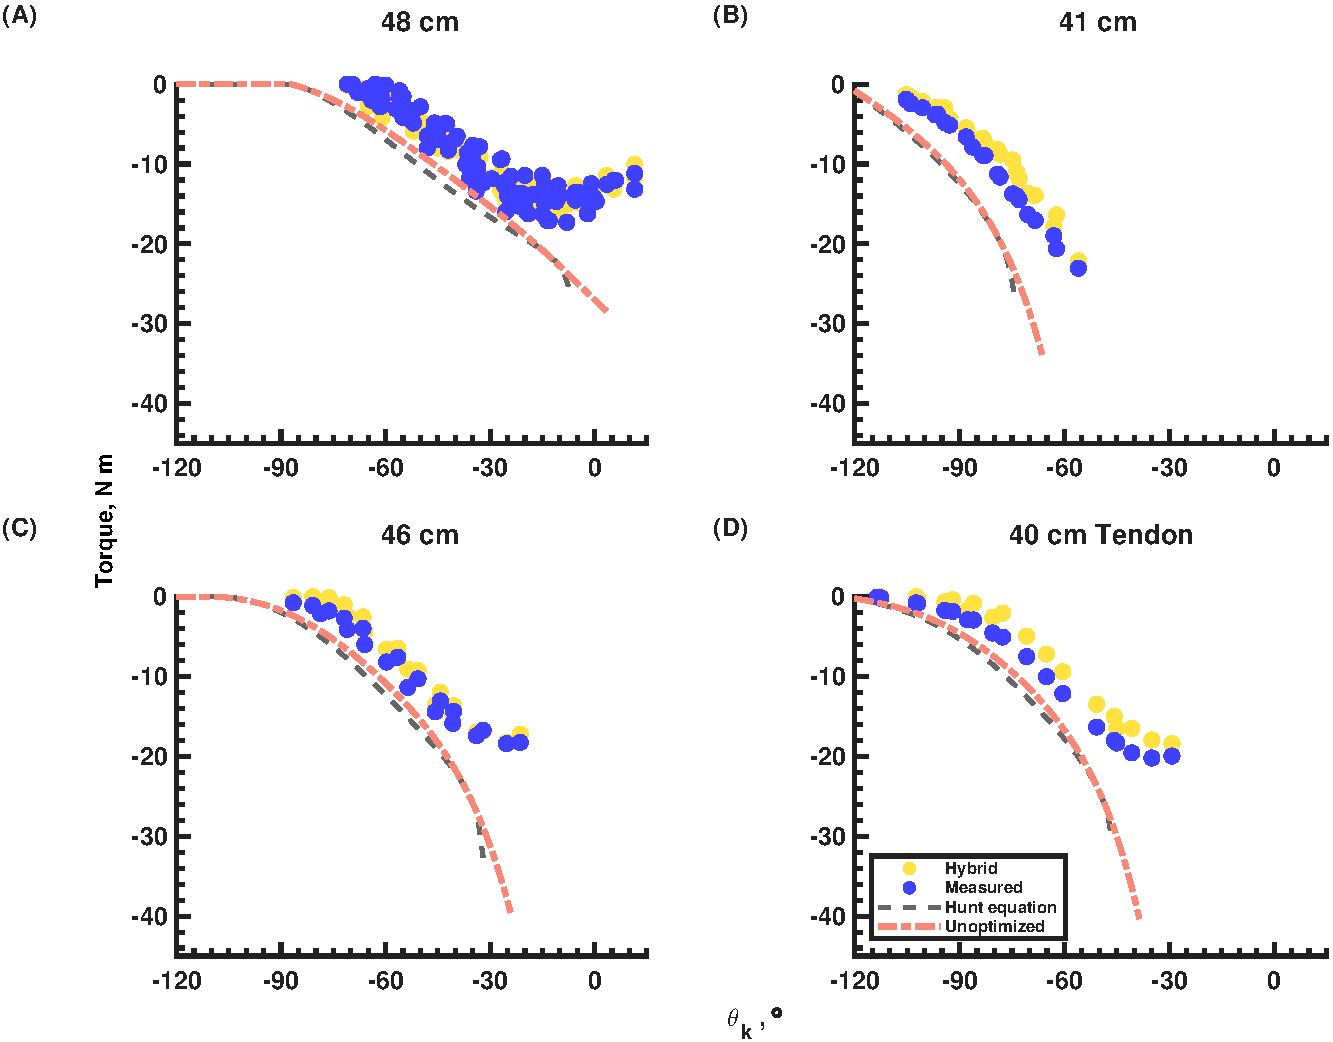
\includegraphics[width=0.8\textwidth]{Figures/FlxPin_preopt_publication.pdf}
\end{center}
\caption{Pinned-knee flexor torque before design-parameter optimization: \textbf{(A)} $l_0=\qty{48.5}{\cm}$, \textbf{(B)} $l_0=\qty{41.0}{\cm}$, \textbf{(C)} $l_0=\qty{45.7}{\cm}$, and \textbf{(D)} $l_0=\qty{40.6}{\cm}$ with a \qty{35}{\mm} tendon. Panels \textbf{(A)} and \textbf{(B)} are training tests; \textbf{(C)} and \textbf{(D)} are validation tests. The legend distinguishes measurements, the Hunt model, the improved BPA model, and the hybrid calculation.}\label{fig:FlxPin}\label{fig:FlxPin_preopt}
\end{figure}

\begin{figure}[htbp]
\begin{center}
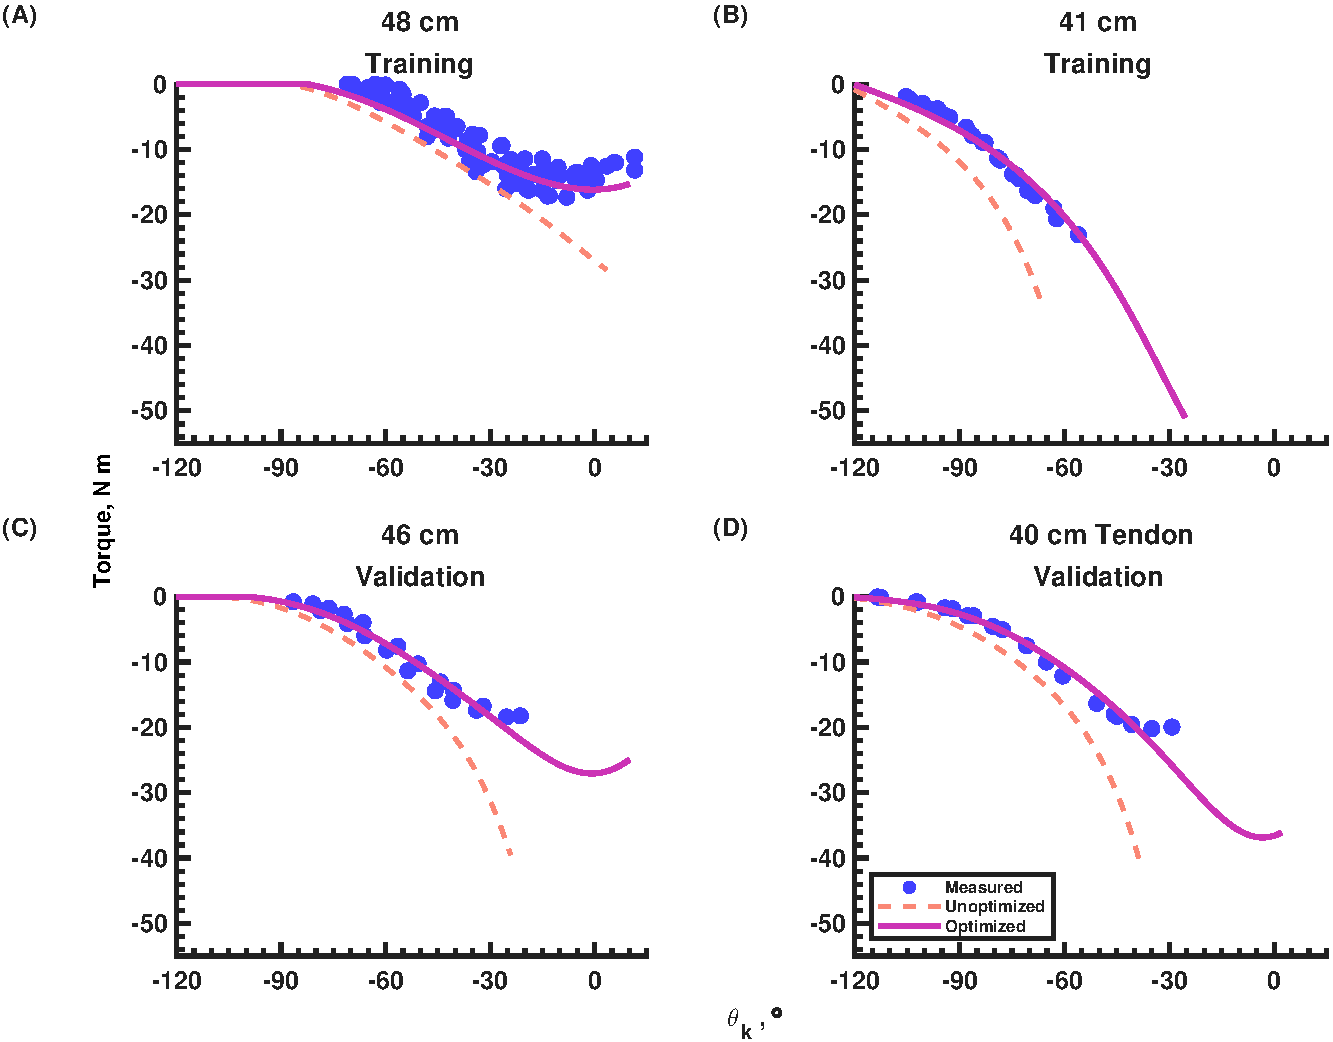
\includegraphics[width=\linewidth,height=0.62\textheight,keepaspectratio]{Figures/FlxPin_optimized_publication.pdf}
\end{center}
\caption{Optimized pinned-knee flexor torque: \textbf{(A)} $l_0=\qty{48.5}{\cm}$, \textbf{(B)} $l_0=\qty{41.0}{\cm}$, \textbf{(C)} $l_0=\qty{45.7}{\cm}$, and \textbf{(D)} $l_0=\qty{40.6}{\cm}$ with a \qty{35}{\mm} tendon. Panels \textbf{(A)} and \textbf{(B)} are training tests; \textbf{(C)} and \textbf{(D)} are validation tests. Circles show measurements, dashed curves the improved BPA model, and solid magenta curves the optimized model.}\label{fig:FlxPin_optimized}
\end{figure}





\subsection{Extensor on Pin Joint}

Two features of the pinned-extensor measurements shaped the extensor identification. First, the measured torque crossed zero at a more extended angle than the prediction, indicating a length offset opposite in sign to the flexor offset. Second, on the $l_{0}=\qty{45.7}{\cm}$ test the hybrid calculation tracked the original prediction closely while the measured torque diverged from both, and the divergence grew with torque as the actuator wrapped over the joint.

The extensor identification of record locks the stiffness pair at the flexor-identified values and solves the two extensor-specific terms: $\chi_{0} = \qty{-6.38}{\mm}$ and $\chi_{3} = 0.158$, so the extensor length offset is close to the flexor offset in magnitude and opposite in sign (Table~\ref{tab:AdoptedXi}). The refit used the six-test identification pool of Section~\ref{sec:identification}, with the \qty{43.6}{\cm}, \qty{43.2}{\cm}-tendon, and \qty{45.7}{\cm} tests in training and the \qty{40.0}{\cm} plain, \qty{40.0}{\cm}-tendon, and \qty{46.5}{\cm} tests held out for validation; Figure~\ref{fig:ExtPin_group} shows the six pool tests at the adopted terms.

\begin{figure}[htbp]
\begin{center}
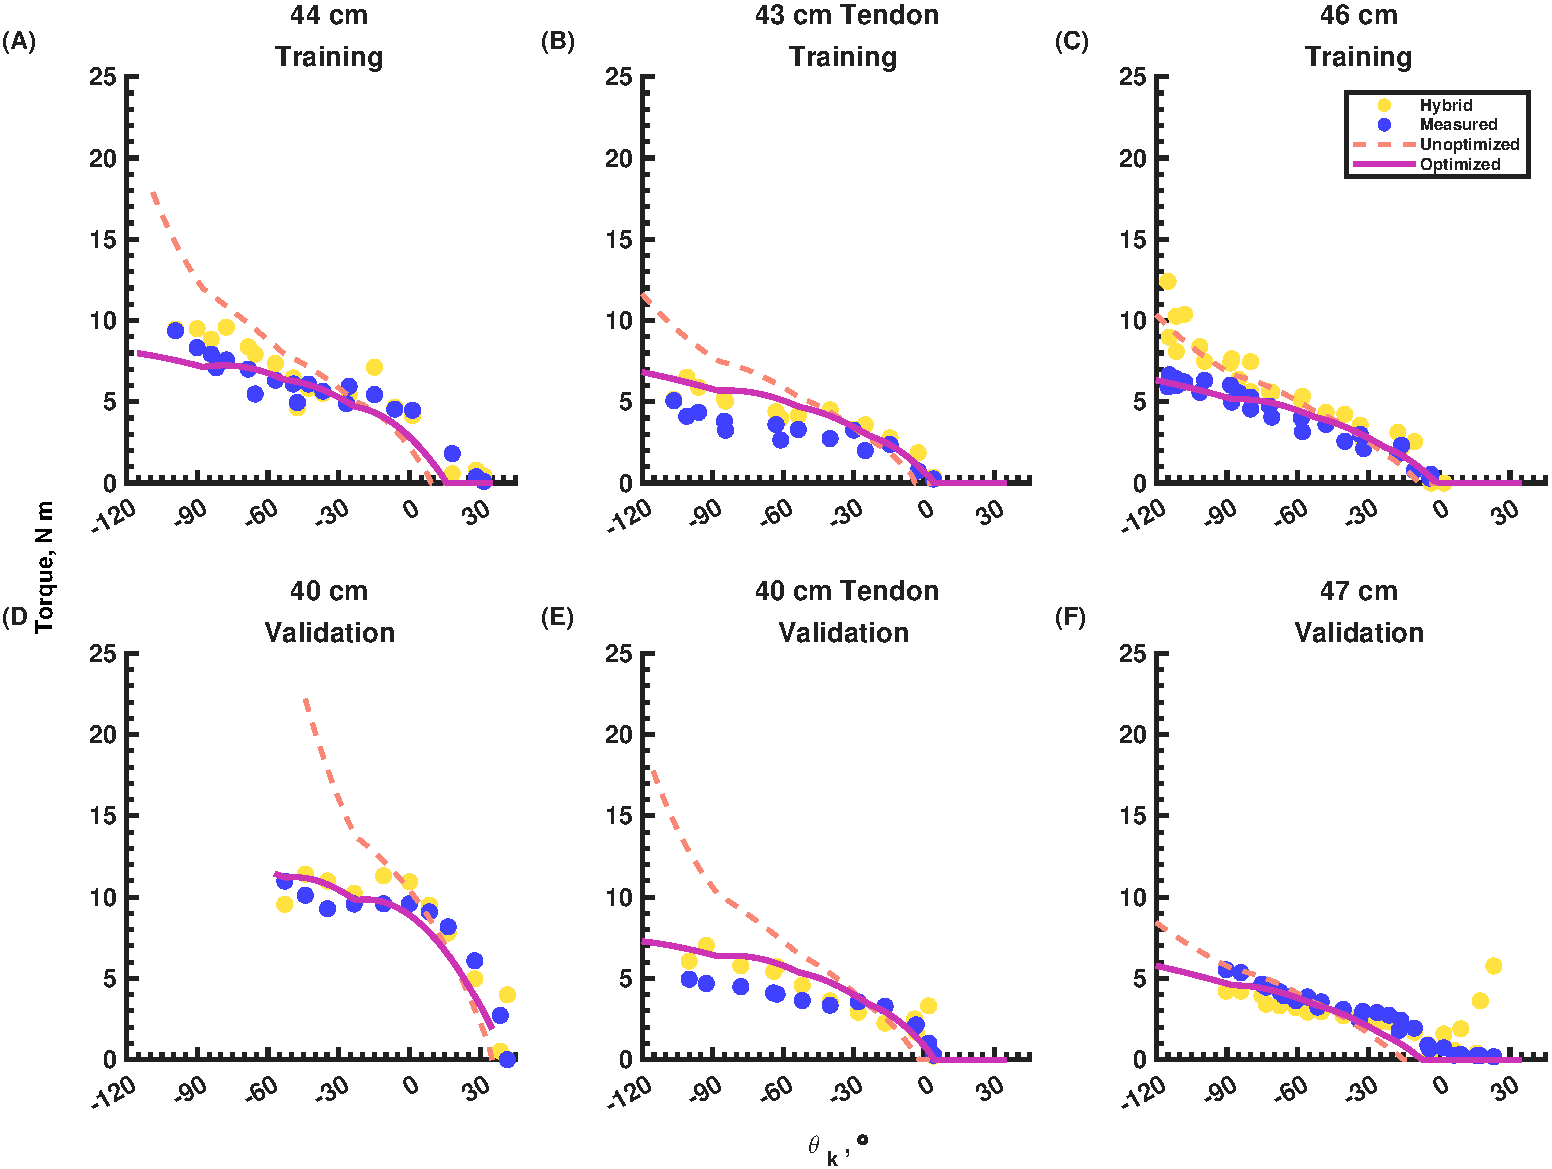
\includegraphics[width=\linewidth,height=0.62\textheight,keepaspectratio]{Figures/ExtPin_complete_publication.pdf}
\end{center}
\caption{Optimized pinned-knee extensor torque: \textbf{(A)} $l_0=\qty{43.6}{\cm}$, \textbf{(B)} $l_0=\qty{43.2}{\cm}$ with a \qty{22}{\mm} tendon, \textbf{(C)} $l_0=\qty{45.7}{\cm}$, \textbf{(D)} $l_0=\qty{40.0}{\cm}$, \textbf{(E)} $l_0=\qty{40.0}{\cm}$ with a \qty{40}{\mm} tendon, and \textbf{(F)} $l_0=\qty{46.5}{\cm}$. Panels \textbf{(A)}--\textbf{(C)} are training tests; \textbf{(D)}--\textbf{(F)} are validation tests. The legend applies to all panels.}\label{fig:ExtPin_group}
\end{figure}

\begin{table}[p]
\centering
\caption{Pinned-knee goodness of fit before and after correction: flexor and extensor. RMSE and maximum residual are in N\,m; FVU is dimensionless.}
\label{tab:FlxPinGof}\label{tab:ExtPinGof}
\begingroup\small\renewcommand{\arraystretch}{1.15}
\noindent\textbf{Flexor}\par\smallskip
\begin{tabular}{@{}cc cccccc@{}}
\toprule
& & \multicolumn{3}{c}{\textbf{Improved BPA}} & \multicolumn{3}{c}{\textbf{Optimized model}} \\
\cmidrule(lr){3-5} \cmidrule(l){6-8}
$\boldsymbol{l_{0}}$ (\unit{\cm}) & $\boldsymbol{l_{\text{ten}}}$ (\unit{\mm}) & \textbf{RMSE} & \textbf{FVU} & \textbf{Max.} & \textbf{RMSE} & \textbf{FVU} & \textbf{Max.} \\
\midrule
\multicolumn{8}{@{}l}{\textbf{Training}} \\
48.5 & -- & 7.617 & 2.1278 & 25.531 & 2.165 & 0.1718 & 5.467 \\
41.0 & -- & 9.694 & 2.1149 & 21.076 & 1.084 & 0.0277 & 1.766 \\
\multicolumn{2}{@{}l}{\hspace*{1em}Mean} & 8.656 & 2.1213 & 23.303 & 1.624 & 0.0998 & 3.617 \\
\midrule
\multicolumn{8}{@{}l}{\textbf{Validation}} \\
45.7 & -- & 8.803 & 1.9380 & 26.264 & 1.368 & 0.0468 & 3.614 \\
40.6 & 35 & 6.373 & 0.5935 & 16.859 & 1.611 & 0.0427 & 5.891 \\
\multicolumn{2}{@{}l}{\hspace*{1em}Mean} & 7.588 & 1.2657 & 21.562 & 1.490 & 0.0447 & 4.752 \\
\bottomrule
\end{tabular}
\par\medskip\noindent\textbf{Extensor}\par\smallskip
\begin{tabular}{@{}cc cccccc@{}}
\toprule
& & \multicolumn{3}{c}{\textbf{Improved BPA}} & \multicolumn{3}{c}{\textbf{Optimized model}} \\
\cmidrule(lr){3-5} \cmidrule(l){6-8}
$\boldsymbol{l_{0}}$ (\unit{\cm}) & $\boldsymbol{l_{\text{ten}}}$ (\unit{\mm}) & \textbf{RMSE} & \textbf{FVU} & \textbf{Max.} & \textbf{RMSE} & \textbf{FVU} & \textbf{Max.} \\
\midrule
\multicolumn{8}{@{}l}{\textbf{Training}} \\
43.6 & -- & 2.437 & 0.9618 & 4.284 & 0.978 & 0.1634 & 1.818 \\
43.2 & 22 & 2.878 & 4.7304 & 4.817 & 1.525 & 1.3270 & 2.481 \\
45.7 & -- & 2.178 & 1.0586 & 4.974 & 0.490 & 0.0535 & 1.206 \\
\multicolumn{2}{@{}l}{\hspace*{1em}Mean} & 2.498 & 2.2503 & 4.692 & 0.997 & 0.5146 & 1.835 \\
\midrule
\multicolumn{8}{@{}l}{\textbf{Validation}} \\
40.0 & -- & 3.092 & 0.5638 & 4.842 & 1.244 & 0.1303 & 2.196 \\
40.0 & 40 & 3.622 & 6.3919 & 7.845 & 1.350 & 0.8878 & 1.890 \\
46.5 & -- & 0.949 & 0.3152 & 2.272 & 0.699 & 0.1714 & 1.559 \\
\multicolumn{2}{@{}l}{\hspace*{1em}Mean} & 2.554 & 2.4236 & 4.986 & 1.098 & 0.3965 & 1.882 \\
\bottomrule
\end{tabular}
\endgroup
\end{table}

\subsection{Extensor on Biomimetic Knee}

We tested the extensor configuration on the biomimetic knee with a $\diameter$\qty{10}{\mm} BPA at $l_{0}=\qty{51.8}{\cm}$. The measured torque fell well below both the original prediction and the hybrid calculation (Figure~\ref{fig:Ext10mm_52cm}). Applying the extensor terms identified on the pinned knee improved the prediction: at the adopted two-stage terms, the optimized model reached an RMSE of \qty{1.1702}{\newton\meter}, an FVU of 0.6681, and a maximum absolute residual of \qty{2.2088}{\newton\meter}, against \qty{3.0322}{\newton\meter}, 4.4856, and \qty{5.5870}{\newton\meter} for the original rigid-body prediction. On this configuration the actuator path passes between the femoral condyles close to the instantaneous center of rotation, a geometry that is difficult to represent with the modeled path (Figure~\ref{fig:Ext10mm_52cm}\textbf{(A)}).

\begin{figure}[htbp]
\begin{center}
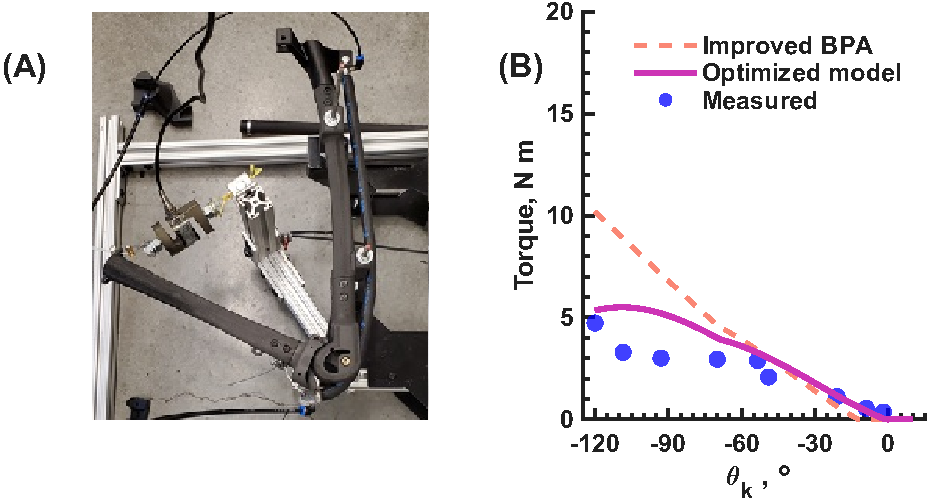
\includegraphics[width=0.9\textwidth]{Figures/Ext10mm_52cm_current_publication.pdf}
\end{center}
\caption{Biomimetic-knee extensor test: \textbf{(A)} apparatus with the BPA passing between the femoral condyles; \textbf{(B)} measured torque, the improved BPA baseline, the optimized model at the adopted terms, and the approximate hybrid calculation for the \qty{10}{\mm}-diameter, \qty{51.8}{\cm} BPA.}\label{fig:Ext10mm_52cm}
\end{figure}

\subsection{Flexor on Biomimetic Knee}

Figure~\ref{fig:FlxGrp} shows the biomimetic-knee flexor measurements and their optimized-model comparisons (Table~\ref{tab:TorqueFit}). Panel \textbf{(A)} presents the $\diameter$\qty{10}{\mm} actuator at $l_{0}=\qty{41.5}{\cm}$ with a \qty{21}{\mm} artificial tendon ($\diameter$\qty{1.5}{\mm} bicycle brake cable wrapped four times), pressurized to \qty{604}{\kPa}; the optimized model reached an RMSE of \qty{2.8002}{\newton\meter}, an FVU of 0.8835, and a maximum absolute residual of \qty{4.1201}{\newton\meter}. Panel \textbf{(B)} presents the $\diameter$\qty{20}{\mm} actuator at $l_{0}=\qty{41.5}{\cm}$ with a \qty{14}{\mm} artificial tendon at \qty{620}{\kPa}, for which the optimized model reached an RMSE of \qty{2.2070}{\newton\meter}, an FVU of 0.0748, and a maximum absolute residual of \qty{3.7320}{\newton\meter}.

The torque of the single $\diameter$\qty{20}{\mm} flexor actuator of panel \textbf{(B)} did not exceed the magnitude of the maximum human isometric flexion torque \citep{delp_interactive_1990,seth_opensim_2018} between \ang{60} and \ang{100} of knee flexion; within a $\pm 20\%$ band about the human mean, it still fell short of human-level torque between \ang{78} and \ang{103} of flexion, the shortfall extending slightly past the upper end of the no-tolerance comparison. Because operating at \qty{620}{\kPa} across the full desired range of motion would load the printed femur beyond its ultimate strength, we also recorded single points at the reduced pressures \qtylist{560;421;325;281}{\kPa}, which show that the desired range of motion is achievable at reduced pressure. This shortfall in flexion torque defines the target that the attachment-route redesign reported in the Discussion addresses.

\begin{figure}[htbp]
\begin{center}
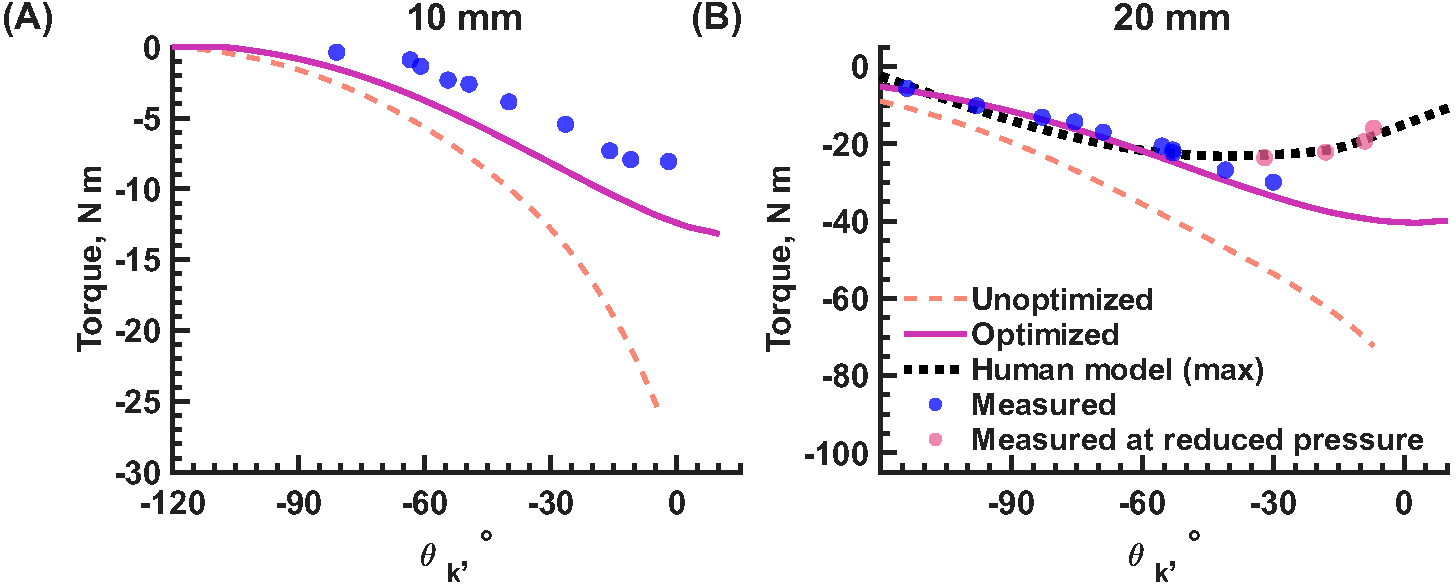
\includegraphics[width=\linewidth]{Figures/Biomimetic_flexor_AB_publication.pdf}
\end{center}
\caption{Biomimetic-knee flexor torque for $l_0=\qty{41.5}{\cm}$ BPAs: \textbf{(A)} \qty{10}{\mm} diameter, \qty{21}{\mm} tendon, and \qty{604}{\kPa}; \textbf{(B)} \qty{20}{\mm} diameter, \qty{14}{\mm} tendon, and \qty{620}{\kPa}. The legend identifies the improved BPA and optimized model predictions, measured torque, and the human reference. Pink markers in \textbf{(B)} show measurements at reduced pressure.}\label{fig:FlxGrp}
\end{figure}

\begin{table}[htbp]
\centering\small
\caption{Biomimetic-knee goodness of fit before and after design-parameter optimization. RMSE and maximum absolute residual (Max.) are in $\mathrm{N\,m}$; FVU is dimensionless.}
\label{tab:TorqueFit}
\begin{tabular}{@{}lrrrrrr@{}}
\toprule
 & \multicolumn{3}{c}{\textbf{Improved BPA}} & \multicolumn{3}{c}{\textbf{Optimized model}} \\
\cmidrule(lr){2-4}\cmidrule(l){5-7}
\textbf{Configuration} & \textbf{RMSE} & \textbf{FVU} & \textbf{Max.} & \textbf{RMSE} & \textbf{FVU} & \textbf{Max.} \\
\midrule
Extensor, $\diameter\qty{10}{\mm}$ & 3.0322 & 4.4856 & 5.5870 & 1.1702 & 0.6681 & 2.2088 \\
Flexor, $\diameter\qty{10}{\mm}$ & 7.4513 & 5.5612 & 13.3163 & 2.8002 & 0.8835 & 4.1201 \\
Flexor, $\diameter\qty{20}{\mm}$ & 14.8064 & 3.3672 & 23.7218 & 2.2070 & 0.0748 & 3.7320 \\
\bottomrule
\end{tabular}
\end{table}


\clearpage
\section{Discussion}\label{sec:discussion}

\subsection{Sources of Error in Isometric Torque Generation}\label{sec:disc_error}

The improved BPA force characterization removes part of the torque-prediction error, but only part (Figure~\ref{fig:FlxPin}). The remainder traces to the test system itself. The isometric system is not rigid: the winch cable, the artificial tendons, and the attachment brackets all bend and stretch under load, and the correction family $\chi_{0}$, $\chi_{1}$, and $\chi_{2}$ was created to represent them. Positioning tolerances, imperfect path modeling, and variation between individual actuators contribute as well.

The combination of high actuator force and a short moment arm makes extensor torque sensitive to attachment deflection and small errors in the routed path. Modeling a BPA that wraps around the knee introduces further geometric approximation. Small moment-arm errors can therefore produce substantial torque errors \citep{young_analyzing_2019}, which is why moment-arm determination receives so much attention in musculoskeletal modeling \citep{brand_model_1982, menegaldo_moment_2004, suderman_moving_2012}. We chose to wrap the BPA around the joint rather than add a patella with a deterministically designed location and friction; the resulting path, which passes between the femoral condyles close to the migrating center of rotation of the biomimetic knee \citep{steele_biomimetic_2018}, resists any straight-line idealization (Figure~\ref{fig:Ext10mm_52cm}\textbf{(A)}). At high flexion, the shorter actuators were also observed to stretch and compress (Figure~\ref{fig:testJigs}\textbf{(C)}), and the same loading occasionally slipped the actuator off the anterior bolt head that holds the femur to the knee, displacing the path by up to $\pm$\qty{20}{\mm} in the $Z$ direction and changing both the force vector and the torque. Supplementary Figure~\ref{fig:extensor_misalign} shows the actuator displacement in top and side views.

The pinned extensor tests exposed one further error source, with a signature distinct from compliance. Figure~\ref{fig:ExtPin_group} shows a deviation between measured and originally predicted torque that widens as the expected torque grows, yet the hybrid calculation matches or exceeds the prediction except at the highest flexion angles. That combination points to a loss of functional muscle length rather than excess compliance, and it is why the wrapping-loss term $\chi_{3}$ was created in Equation~(\ref{eq:deltaL}). Bent over the joint, the actuator behaves like a beam, and the wrapped arc stops contributing usable contraction, so the actuator behaves as if it were more contracted than it physically is; this is the fictive strain of Section~\ref{sec:fictive_contraction}, and Section~\ref{sec:adopted_identification} quantifies it.

The pinned-knee tests distinguish actuator-force error from errors introduced by attachment compliance and routed geometry. Applying the identified terms to the biomimetic knee then tests their usefulness when the ICR and moment arm change with knee angle. This sequence links the correction terms to measured mechanisms and identifies the remaining limits of torque prediction.

\subsection{Identified Design Parameters}\label{sec:adopted_identification}

The adopted correction terms are listed in Table~\ref{tab:AdoptedXi}.

\begin{table}[H]
\caption{Adopted correction terms. The effective stiffness pair is shared; $\chi_3$ was identified on the extensor and is applied to wrapping in the redesigned flexor.}
\label{tab:AdoptedXi}
\begingroup
\renewcommand{\arraystretch}{1.4}%
\fontsize{10pt}{12pt}\selectfont
\begin{tabular}{@{}lcccc@{}}
\toprule
\textbf{Configuration} & $\boldsymbol{\chi_{0}}$ (\unit{\metre}) & $\boldsymbol{\chi_{1}}$ (\unit{\N\per\metre}) & $\boldsymbol{\chi_{2}}$ (\unit{\N\per\metre}) & $\boldsymbol{\chi_{3}}$ \\
\midrule
Flexor configuration & \num{+3.94e-3} & \num{3.998e4} & \num{1.473e4} & -- \\
Extensor configuration & \num{-6.38e-3} & \num{3.998e4} & \num{1.473e4} & \num{0.158} \\
\bottomrule
\end{tabular}
\endgroup
\end{table}

Each term has a direct physical reading. The offsets $\chi_{0}$ correct the effective muscle length by a constant, and the flexor and extensor offsets carry opposite signs. The fitted stiffness pair describes effective attachment compliance rather than the beam stiffness of any single part: it lumps the two attachment brackets together with the fixtures and the winch cable, which is why one pair can serve both configurations once the extensor refit locks it. The wrapping factor $\chi_{3}$ scales the usable length that fictive strain removes, $\Delta l = \chi_{3}\, R\, \abs{\theta_{\text{wrap}} - \theta_{\text{k}}}\, \zeta^{2}$ with $\zeta = 1 - \varepsilon^{*}$ (Equations~(\ref{eq:deltaL}) and (\ref{eq:comp})). Because $\varepsilon^{*}$ is normalized by the unloaded \qty{620}{\kPa} contraction $\varepsilon_{620}$ of the free actuator, the loss is expressed in fictive-contraction units: it vanishes as the actuator approaches full contraction, where $\zeta \to 0$, and grows quadratically toward resting length, where the unbent actuator would otherwise produce its largest force. The wrapping radii are fixed by the route geometry rather than fitted: the pinned-extensor identification evaluates two contact arcs of wrapping radii $R = \qty{12}{\mm}$ and $R = \qty{40}{\mm}$, and the biomimetic-knee test with the \qty{10}{\mm} extensor uses a wrap radius of \qty{25}{\mm}, so $\chi_{3} = 0.158$ scales a physical arc of known size.

Table~\ref{tab:FlxPinGof} quantifies the improvement after optimizing $\chi_0$--$\chi_3$. For the pinned flexor, mean RMSE decreases from \qty{8.66}{\newton\meter} to \qty{1.62}{\newton\meter} on the training tests and from \qty{7.59}{\newton\meter} to \qty{1.49}{\newton\meter} on the validation tests. For the pinned extensor, the corresponding means decrease from \qty{2.50}{\newton\meter} to \qty{1.00}{\newton\meter} and from \qty{2.55}{\newton\meter} to \qty{1.10}{\newton\meter}. In each comparison, the baseline uses the same improved BPA force model and routed geometry with the correction terms disabled. The optimized model improves RMSE for every identification test, although the \qty{43.2}{\cm} tendon extensor retains FVU above unity. The biomimetic-knee comparisons in Table~\ref{tab:TorqueFit} provide a separate assessment of transfer beyond the pinned-knee configurations.

The solver was selected to match each optimization task. The identification retains the genetic multiobjective solver, an elitist nondominated-sorting genetic algorithm, because the Pareto front it returns is what the holdout-validation procedure selects from. The route redesign is served by the surrogate-plus-pattern-search pipeline of Section~\ref{sec:route_redesign}, a surrogate-assisted global search refined by a derivative-free mesh-adaptive pattern search, because a single scalar cost is optimized there and each route evaluation is expensive.

\subsection{Route Redesign and Physical Validation}\label{sec:route_redesign_results}

\subsubsection{Route Redesign and Cost Functions}

The flexor and extensor routes use different terms in the common objective of Equation~\eqref{eq:opt_cost}:
\begin{align}
J_{\mathrm{flx}} =\;& 10^{5}J_{\text{worst}} + 10^{3}J_{\text{torque}} + 10^{-2}J_{\text{shape}} + J_{\text{off}} + J_{\text{rest}} + J_{\text{strain,hi}} \nonumber\\
& + J_{\text{strain,lo}} + J_{\text{wrap}} + J_{\text{geom}} + J_{\text{len}} + J_{\text{anchor}},
\label{eq:opt_cost_flx}\\[4pt]
J_{\mathrm{ext}} =\;& 10^{5}J_{\text{worst}} + 10^{3}J_{\text{torque}} + J_{\text{over}} + J_{\text{rest}} + J_{\text{strain,hi}} \nonumber\\
& + J_{\text{strain,lo}} + J_{\text{contr}} + J_{\text{geom}} + J_{\text{len}}.
\label{eq:opt_cost_ext}
\end{align}
Here $J_{\text{shape}}$ penalizes torque-curve disagreement, $J_{\text{off}}$ off-axis torque, $J_{\text{rest}}$ infeasible resting length, $J_{\text{strain,hi}}$ and $J_{\text{strain,lo}}$ strain-limit violations, $J_{\text{wrap}}$ failure to release a wrap, $J_{\text{anchor}}$ attachment displacement, $J_{\text{over}}$ torque overshoot, and $J_{\text{contr}}$ excessive contraction. Geometric and length regularizers retain the seed neighborhood. The cam formulation additionally rewards worst-angle torque margin and penalizes abrupt changes in moment arm and displacement from the initial cam profile. These additions seek usable torque capacity while preserving feasible actuator travel.

The redesign addresses the single-actuator shortfall documented in the Results: one BPA per route does not reach the human flexor envelope through the mid-flexion range. Every redesigned configuration therefore carries two $\diameter$\qty{20}{\mm} BPAs per route, a \qty{620}{\kPa} pressure ceiling, and a maximum usable contraction of 0.255 in the force model, and every family was produced by the procedure of Section~\ref{sec:route_redesign} under the adopted correction terms of Table~\ref{tab:AdoptedXi}. The targets are maximum-isometric torque profiles computed on the Gait2392 lower-extremity model \citep{delp_opensim_2007, seth_opensim_2018}, the vastus medialis for the extensor and the biceps femoris short head for the flexor, each enlarged by a required \qty{5}{\percent} overshoot margin so that a route merely touching the target at any angle is rejected, and the redesign itself runs on the robot-body model derived from it. Knee angles are negative in flexion throughout this section, and Supplementary Figure~\ref{fig:RouteVariants} graphs the four redesigned route families against their human-scaled requirements.

The direct extensor route exceeds the human envelope in magnitude at every angle, with zero shortfall points. Across the design range, the predicted two-BPA torque spans \qty{35.45}{\newton\meter} to \qty{109.4}{\newton\meter} against a human-scaled requirement of \qty{20.25}{\newton\meter} to \qty{50.32}{\newton\meter}, and the required overshoot is consumed as the thinnest margin exactly as designed, $+5.02$~\% at the worst-case angle of \ang{-20.2}. The route respects the wrap-release schedule of the route-elimination rule, releasing its six sequential contacts at knee angles of \ang{-89.8}, \ang{-55.7}, \ang{-47.8}, \ang{-20.2}, \ang{6.1}, and \ang{7.4}, and the optimized design places the femur-side origin at $(40.0, 137.0, 0)$~mm and the tibial insertion at $(34.4, -197.1, 0)$~mm, with a resting length of \qty{827.7}{\mm} and \qty{36.8}{\mm} of tendon.



The extensor route was then redesigned once more by allowing the tibial-side route points to trace a cam profile, and this cam redesign is the current extensor design. The cam increases the torque margin relative to the direct route. On the final geometry, which folds the optimizer winner together with a verified adjustment of the distal route point and tendon length, the minimum torque margin is $+30.83$~\% with respect to the required envelope and $+39.77$~\% with respect to the plain human target; the unadjusted optimizer solution carried $+31.30$~\% and $+42.34$~\% at the same checks. The pressure required to meet the envelope spans \qty{269}{\kPa} to \qty{507}{\kPa} over the range of motion, comfortably above the \qty{150}{\kPa} regulated floor of the valve manifold that supplies the hardware, so the remaining pressure is a design resource. The tibial wrap follows a bend radius of \qty{96.9}{\mm}, the guiding route point clears the femoral-condyle envelope by \qty{43.1}{\mm} at \ang{10} of knee extension, and the moment arm spans \qty{59.4}{\mm} to \qty{102.8}{\mm} with a mean of \qty{72.4}{\mm} (Supplementary Figure~\ref{fig:ExtensorRoute_redesigned}).

The flexor redesign uses two staggered BPA routes rather than a single shared route. The first actuator's route is carried directly as design variables, its origin on the femur and its insertion on the tibia, and the second actuator's endpoints are derived from it by an offset-preserving endpoint rule: the second insertion mirrors the first across the mid-sagittal plane, and the second origin is placed so that the second route spans the same origin-to-insertion offset as the first, which keeps the two routes from crossing. Each route is then rebuilt by the route solver, so the second carries its own wrap point and its own tibial and femoral-condyle clearance state rather than inheriting the first's, with condyle clearance enforced in the nonlinear constraints. In the design of record the first route clears the tibial envelope at every angle and never wraps, while the second rides its standoff only within about \ang{5} of full extension before the wrap releases. The design meets the flexor target with a minimum margin fraction of 0.0501 against the required 0.05. Its predicted knee-axis torque spans \qty{-81.23}{\newton\meter} to \qty{-3.864}{\newton\meter} against the human-scaled requirement of \qty{-23.16}{\newton\meter} to \qty{-2.461}{\newton\meter} (peak magnitude \qty{23.16}{\newton\meter}), again exceeding the envelope at every angle. The flexor prediction applies the adopted correction terms, including the wrapping factor identified on the extensor configuration: where a route's wrap is active, the actuator loses usable length through the same wrapping mechanism, and the extensor-identified $\chi_{3}$ was applied to it unchanged, a transfer evaluated in the redesigned flexor's isometric tests.

\subsubsection{Physical Validation Against Human Torque}

The redesigned cam-assisted extensor route was tested at nine isometric positions from \ang{-119} to \ang{5}, at pressures of \qtyrange{256}{488}{\kPa}. Figure~\ref{fig:Ext20mm} compares measured torque with the pressure-specific model prediction, the optimized \qty{620}{\kPa} curve, and the vastus medialis reference.



All nine extensor measurements meet or exceed the human reference at the tested angles, with torque margins of \qtyrange{0.24}{3.52}{\newton\meter}. Measured torque exceeds the pressure-specific prediction at eight angles, by up to \qty{13.75}{\newton\meter}; at \ang{-86.5}, the measurement exceeds the human reference and is \qty{2.06}{\newton\meter} below the pressure-specific prediction. The discrete measurements support capacity at those configurations; they do not measure a continuous full-pressure envelope.

The redesigned flexor route was then validated physically on the same stand with the two $\diameter$\qty{20}{\mm} actuators of the design of record at $l_{0}=\qty{56.2}{\cm}$ (Figure~\ref{fig:redesign_validation}\textbf{(B)}). The original rigid-body prediction of this design at \qty{620}{\kPa} reaches a peak torque magnitude of \qty{190.3}{\newton\meter}, while the optimized model, carrying the length offset, attachment compliance, and wrapping loss identified on the pinned knee, reaches \qty{91.9}{\newton\meter}. Fifteen isometric measurements span \ang{-119} to \ang{5} at hung loads of \qtyrange{11.1}{106}{\newton} and gauge pressures of \qtyrange{226.5}{638}{\kPa}, with the measured wrench carried to the moving knee center by the same adjoint transform as the identification data; the measured torque magnitude met or exceeded the human target at every point, with margins from \qty{0.42}{\newton\meter} at \ang{-105} to \qty{17.0}{\newton\meter} at \ang{-14}. The discrete measurements establish capacity at the measured configurations; they do not establish agreement with the optimized full-pressure prediction throughout the range.

The installed flexor BPAs had measured resting lengths of \qtylist{561;560}{\mm} and tendon lengths of \qtylist{28;30}{\mm}, respectively; the extensors had resting lengths of \qtylist{828;826}{\mm} and tendon lengths of \qtylist{92;85}{\mm}. These measurements are distinct from the shared prediction inputs: flexor resting length \qty{561.49}{\mm} with an effective \qty{5.00}{\mm} tendon parameter after the fitting adjustment, and extensor resting length \qty{827.74}{\mm} with the approximate \qty{92.49}{\mm} tendon parameter. The plotted predictions retain those design inputs, and the flexor plot retains its nominal \qty{562}{\mm} label.

\begin{figure}[htbp]
\centering
\makebox[\linewidth][l]{\textbf{(A)}}\par
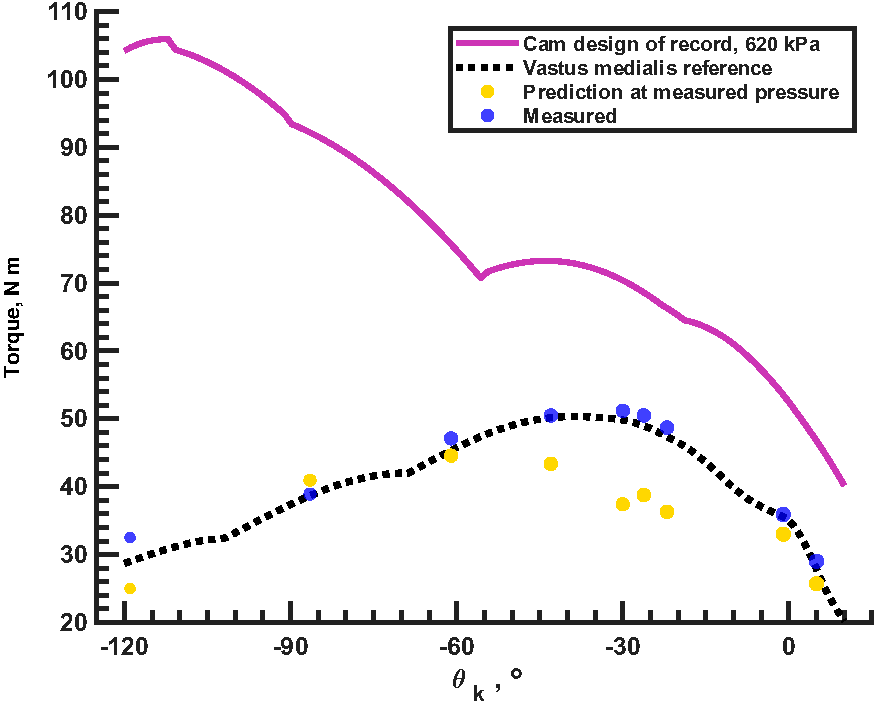
\includegraphics[width=0.86\linewidth,height=0.32\textheight,keepaspectratio]{Figures/Ext20_current_publication.pdf}
\par\medskip
\makebox[\linewidth][l]{\textbf{(B)}}\par
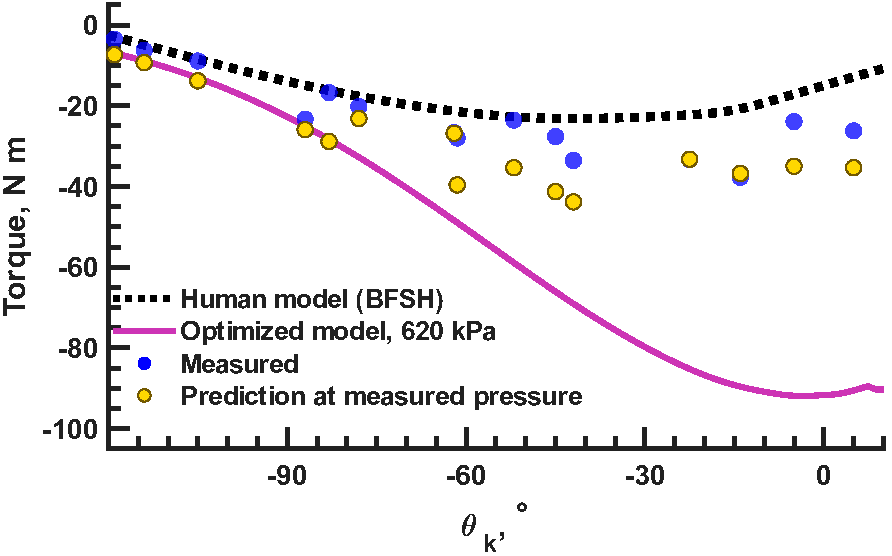
\includegraphics[width=0.86\linewidth,height=0.32\textheight,keepaspectratio]{Figures/Redesigned_flexor_pressure_publication.pdf}
\caption{Physical validation of redesigned two-BPA knee routes. \textbf{(A)} Cam extensor: nine measurements, pressure-specific predictions, the optimized \qty{620}{\kPa} curve, and the vastus medialis reference; marker area scales with pressure. \textbf{(B)} Flexor (nominal \qty{562}{\mm} plot label): fifteen measurements, pressure-specific predictions, the optimized \qty{620}{\kPa} curve, and the biceps femoris short-head reference. Both configurations use \qty{20}{\mm} BPAs.}
\label{fig:Ext20mm}\label{fig:redesign_validation}
\end{figure}

The knee redesign establishes the force--travel and geometric constraints used below to assess transmissions at other actuator sites. The whole-leg comparison evaluates saved configurations on the inherited robot routing; it does not demonstrate that every attachment route has been redesigned or physically validated.

\subsection{Whole-Leg Capability Against Human Torque Surfaces}\label{sec:capability_survey}

With improved torque prediction and route-design methods in place, we revisited the robot-leg configurations of \citet{bolen_determination_2019}. The expanded design search varies parallel actuator count and transmission ratio and re-solves actuator and tendon lengths on the inherited routing. Table~\ref{tab:CapabilitySurvey} summarizes how the selected configurations improve coverage of the human torque requirements.

The reverse-pulley comparison evaluated soleus and tibialis anterior at the ankle, biceps femoris short head at the knee, medial gastrocnemius across the knee and ankle, and rectus femoris across the hip and knee. Sizes were re-solved for each combination of parallel BPAs and tackle line parts, because the required actuator contraction and tendon take-up change with the transmission. Comparisons below use \qty{620}{\kPa}. Each biarticular evaluation fixes the adjacent joint, so a favorable result in one evaluation plane does not establish performance across both joints.

At matched net force, increased tackle travel extended the angle range meeting the human torque requirement. Tibialis anterior increased from \ang{48.1} with one direct-drive BPA to \ang{56.9} with two BPAs through a two-part tackle and \ang{59.8} with four BPAs through a four-part tackle. Medial gastrocnemius increased from \ang{21.7} to \ang{65.0} and \ang{119.2}, respectively. Soleus remained below its human target for all evaluated transmissions: increasing travel could not compensate for its force shortfall. These results motivate evaluating both torque coverage and the ability to maintain active force over the joint domain.

The capability survey grades each actuator against the same-named single muscle of the Gait2392 model \citep{delp_opensim_2007,seth_opensim_2018} on a $5\times5$ grid of two joint coordinates. The hip adduction domain is clipped by its flexion-dependent envelope. A cell meets the requirement when the BPA is taut and its torque has the human torque's sign and at least its magnitude. The coverage metric is the fraction of included grid cells meeting that condition; the aggregate is the unweighted mean of the per-actuator fractions, not a continuous-area integral or a whole-leg torque sum.

The BPA force model is evaluated at \qty{620}{\kPa} \citep{bolen_2026}. The comparison includes all 27 actuator sites (Supplementary Table~\ref{tab:survey_dofs_sizes}). The baseline uses the master's-era attachment routing at unity transmission; its eight nominal \qty{40}{\mm} sites are evaluated with four parallel \qty{20}{\mm} BPAs, while the other sites use the survey's base configuration. The updated side selects the saved transmission-ladder winner at each site, with actuator length and tendon length re-solved per configuration. It retains the same underlying attachment routing and the original diameter specification, including \qty{40}{\mm} actuators at those eight sites. The comparison therefore combines transmission, actuator sizing, and the baseline diameter substitution; it does not isolate an effect of attachment placement or compare two all-\qty{20}{\mm} assemblies.

Active-force coverage is the fraction of included grid cells with positive insertion tension, excluding slack or infeasible configurations. It does not require the torque to match the human reference. Both coverage measures are calculated for each actuator and then averaged equally across the 27 sites. Table~\ref{tab:CapabilitySurvey} reports the resulting means.

The mean fraction meeting the human torque requirement increases from \qty{37.28}{\percent} for the baseline to \qty{65.19}{\percent} for the saved transmission configurations, improving at 23 sites and tying at four. Mean active-force coverage increases from \qty{92.44}{\percent} to \qty{98.81}{\percent}. The higher active-force coverage shows that the transmission configurations maintain tension over more of the graded domain, while the lower torque coverage shows that positive tension alone is insufficient to meet the human torque requirement.

\begin{table}[htbp]
\centering
\begingroup
\fontsize{10pt}{12pt}\selectfont
\caption{Mean torque and active-force coverage across 27 actuator sites at \qty{620}{\kPa}.}
\label{tab:CapabilitySurvey}
\begin{tabular}{@{}lcc@{}}
\toprule
\textbf{Configuration} & \textbf{Human torque met (\%)} & \textbf{Active force (\%)} \\
\midrule
Baseline & 37.28 & 92.44 \\
Transmission configurations & 65.19 & 98.81 \\
\bottomrule
\end{tabular}
\endgroup
\end{table}

\subsection{Design Factors for Isometric Torque}\label{sec:design_factors}

Isometric joint-torque design couples moment arm, actuator contraction, and attachment compliance. A larger moment arm increases torque per unit force but also increases the tendon excursion required over a given joint rotation. The cam-assisted extensor illustrates this trade-off: its moment arm spans \qtyrange{59.4}{102.8}{\mm}, compared with \qtyrange{44.9}{61.2}{\mm} for the direct route, while its required pressure remains between \qty{269}{\kPa} and \qty{507}{\kPa} against a \qty{620}{\kPa} ceiling. The additional torque capacity therefore comes from altered routing and travel requirements, with a corresponding departure from the original biomimetic geometry. These quantities should be evaluated together when selecting an attachment route.

These factors situate our work among musculoskeletal robot legs. Multifilament muscle routing has produced human-scale lower limbs \citep{kurumaya_musculoskeletal_2016}, anthropomorphic arms \citep{hitzmann_anthropomorphic_2018}, and full human-mimetic humanoids \citep{asano_musculoskeletal_2019}, and tendon-driven bodies have supported investigations from reflexive hopping \citep{liu_robotic_2018} to human-like manipulation \citep{chen_realizing_2019} and cognitive locomotion \citep{schilling_adaptive_2022}. Linkage-based knees manage the moment-arm problem geometrically \citep{romero_four-bar_2020}, reviews of dynamic multilegged robots treat actuation routing as a first-order design decision \citep{he_mechanism_2020}, and tunable-compliance actuators make fixture compliance a design element rather than an error source \citep{leibach_development_2020}. What these designs share with ours is the recognition that the attachment route, not the actuator alone, sets the deliverable torque. What the optimized model adds is a quantitative accounting of the compliance and wrapping losses along that route, so that a route can be designed against a torque target rather than checked after the fact. \citet{morrow_optimization_2020} optimized artificial-muscle placement on a bipedal robot with a rigid-body torque model, and the correction terms quantified here are the physics such rigid-body placements leave unmodeled.

The correction family also complements the BPA force-modeling literature. Static models of the actuator in isolation, from the classical McKibben analyses \citep{chou_measurement_1996} through approximation formulas \citep{sarosi_new_2012} to geometrically grounded models of the Festo muscle \citep{martens_modeling_2017, tondu_static_2022}, describe the actuator itself; none of them carries attachment compliance, length offsets, or wrapping losses into a joint-torque prediction. The correction terms used here attach to the force characterization of \citet{bolen_2026} and represent the transmission losses encountered at the joint. The shared-pair extensor comparison and the physical redesigned-route tests provide specific checks of transfer; they do not establish unrestricted transfer to other hardware.

\subsection{Limitations and Future Work}\label{sec:limitations}

 The correction terms are identified for this test stand, these knee configurations, and these actuator families. Other joints or actuator types should repeat the two-stage procedure rather than reuse the values. Reverse-pulley transmissions can increase internal reaction loads relative to the delivered tendon force. Pulley mounts, brackets, and cables must therefore be checked against the internal forces, including the possibility of excessive deflection or component failure. Transfer to other systems requires validation against their measured torque. 

Isometric testing measures torque at fixed joint positions and therefore establishes a static capacity envelope. Isokinetic testing controls joint speed, allowing torque to be compared across angles at a defined velocity and repeated at several velocities. For this robot, those tests would show how contraction rate, pressure regulation, and changing moment arm affect the torque available during movement, and whether the static design margin remains adequate. Isotonic testing maintains a prescribed external load while the actuator shortens; it would assess shortening speed, achievable excursion, and the ability to support a load through the movement. Loading and unloading sequences would quantify hysteresis, while pressure-step tests would characterize pneumatic response. A torque-controlled motor and a less compliant loading connection would reduce winch slack and permit controlled-speed and controlled-load tests on the same rig. Together, these measurements would identify the additional dynamics needed to extend the static model to movement and load-bearing control.

\section{Conclusion}\label{sec:conclusion}

Isometric knee-torque measurements on pinned and biomimetic test stands showed that actuator force characterization alone does not determine delivered joint torque. A hybrid calculation using measured muscle length and moment arm helped separate force-model error from routing and attachment effects. The corrected torque model represents a constant length offset, effective attachment compliance, and an empirical wrapping loss. A two-stage identification shares one stiffness pair across flexor and extensor configurations and reduces prediction error on the validation tests.

Route redesign under the optimized model produces configurations with two $\diameter$\qty{20}{\mm} BPAs that meet the selected human-muscle torque targets over their design grids, with the required \qty{5}{\percent} margin. The cam-assisted extensor increases predicted torque headroom while reducing the required operating pressure. Physical tests meet or exceed the respective human targets at all 15 measured flexor points and all nine measured extensor points. These measurements validate the tested isometric configurations; dynamic loading and transfer to other joints remain to be evaluated. Together, the identified design factors and the corrected routing calculations support more successful first-pass designs by accounting for transmission losses before hardware is built.

\section*{Resource Identification Initiative}
\begin{itemize}
    \item MATLAB (RRID:SCR\_001622)
    \item OpenSim (RRID:SCR\_002683)
    \item Arduino UNO (RRID:SCR\_017284)
\end{itemize}

%To take part in the Resource Identification Initiative, please use the corresponding catalog number and RRID in your current manuscript. For more information about the project and for steps on how to search for an RRID, please click \href{http://www.frontiersin.org/files/pdf/letter_to_author.pdf}{here}.


\section*{Conflict of Interest Statement}
The authors declare no conflicts of interest. The funders had no role in the design of the study; in the collection, analysis, or interpretation of data; in the writing of the manuscript; or in the decision to publish the results.

\section*{Author Contributions}
Conceptualization, B.B. and C.M.; Methodology, B.B., C.M., and A.H.; Software, B.B., C.M., and L.B.; Validation, B.B. and A.H.; Formal Analysis, B.B.; Investigation, B.B., C.M., and L.B.; Resources, B.B., L.B., and A.H.; Data Curation, B.B.; Writing -- Original Draft Preparation, B.B.; Writing -- Review \& Editing, B.B., C.M., L.B., and A.H.; Visualization, B.B. and A.H.; Supervision, B.B. and A.H.; Project Administration, B.B. and A.H.; Funding Acquisition, A.H.

\section*{Funding}
Research for this article was funded by the Department of Mechanical and Materials Engineering at Portland State University, the National Science Foundation (NSF) grant for NeuroNex: Communication, Coordination, and Control in Systems (C3NS) 2015317 and NSF grant 1943483. 

%Details of all funding sources should be provided, including grant numbers if applicable. Please ensure to add all necessary funding information, as after publication this is no longer possible.

\section*{Acknowledgments}
The authors would like to acknowledge the contribution of Alex Steele, who designed the initial biomimetic 4-bar knee linkage we used for the test. He gave us solid models, built a 3D prototype, and let us break said prototype. His prompt and thoughtful responses to our questions about the previous design was very much appreciated. The authors would also like to thank Jasmine Bradley for her help reworking the figures in the results section. As a visual designer, her contributions improved the aesthetic quality and accessibility of the images. 
%This is a short text to acknowledge the contributions of specific colleagues, institutions, or agencies that aided the efforts of the authors.

\section*{Supplemental Data}
Supplemental Data provides the biomimetic fit statistics, attachment and routing coordinates, contact-release method, configuration-survey coordinates, and supporting figures of route torque, actuator slippage, and cam geometry.
 
 %\href{http://home.frontiersin.org/about/author-guidelines#SupplementaryMaterial}{Supplementary Material} should be uploaded separately on submission, if there are Supplementary Figures, please include the caption in the same file as the figure. LaTeX Supplementary Material templates can be found in the Frontiers LaTeX folder.

\section*{Data Availability Statement}
The data sets are available from the authors upon reasonable request.

%The datasets [GENERATED/ANALYZED] for this study can be found in the [NAME OF REPOSITORY] [LINK].

% Please see the availability of data guidelines for more information, at https://www.frontiersin.org/about/author-guidelines#AvailabilityofData

\bibliographystyle{Frontiers-Harvard} %  Many Frontiers journals use the Harvard referencing system (Author-Date), to find the style and resources by journal: https://zendesk.frontiersin.org/hc/en-us/articles/360017860337-Frontiers-Reference-Styles-by-Journal. For Humanities and Social Sciences articles please include page numbers in the in-text citations 
%\bibliographystyle{Frontiers-Vancouver} % Many Frontiers journals use the numbered referencing system (Author-date), to find the style and resources by journal: https://zendesk.frontiersin.org/hc/en-us/articles/360017860337-Frontiers-Reference-Styles-by-Journal
\bibliography{BolenFrontiers22}

%%% Make sure to upload the bib file along with the tex file and PDF
%%% Please see the test.bib file for some examples of references

\clearpage


%%% Please be aware that for original research articles we only permit a combined number of 15 figures and tables, one figure with multiple subfigures will count as only one figure.
%%% Use this if adding the figures directly in the mansucript, if so, please remember to also upload the files when submitting your article
%%% There is no need of adding the file termination, as long as you indicate where the file is saved. In the examples below the files (logo1.eps and logos.eps) are in the Frontiers LaTeX folder
%%% If using *.tif files convert them to .jpg or .png
%%%  NB logo1.eps is required in the path in order to correctly compile front page header %%%

%Frontiers requires figures to be submitted individually, in the same order as they are referred to in the manuscript. Figures will then be automatically embedded at the bottom of the submitted manuscript. Kindly ensure that each table and figure is mentioned in the text and in numerical order. Figures must be of sufficient resolution for publication \href{https://www.frontiersin.org/about/author-guidelines#ImageSizeRequirements}{see here for examples and minimum requirements}. Figures which are not according to the guidelines will cause substantial delay during the production process. Please see \href{https://www.frontiersin.org/about/author-guidelines#FigureRequirementsStyleGuidelines}{here} for full figure guidelines. Cite figures with subfigures as figure \ref{fig:2}B.

%%% If you are submitting a figure with subfigures please combine these into one image file with part labels integrated.
%%% If you don't add the figures in the LaTeX files, please upload them when submitting.
%%% Frontiers will add the figures at the end of the provisional pdf automatically
%%% The use of LaTeX coding to draw Diagrams/Figures/Structures should be avoided. They should be external callouts including graphics.



%Tables should be inserted at the end of the manuscript. Please build your table directly in LaTeX.Tables provided as jpeg/tiff files will not be accepted. Please note that very large tables (covering several pages) cannot be included in the final PDF for reasons of space. These tables will be published as \href{http://www.frontiersin.org/about/author-guidelines#SupplementaryMaterial}{Supplementary Material} on the online article page at the time of acceptance. The author will be notified during the typesetting of the final article if this is the case. 


\end{document}
